\documentclass[notes]{beamer}

\usetheme{Darmstadt}
\usepackage{lmodern}% http://ctan.org/pkg/lm
\usepackage{amsthm,amstext,amsfonts,bm,amssymb}

\mode<presentation>
%\useoutertheme{smoothbars}
\useinnertheme[shadow=true]{rounded}
\usecolortheme{whale}
\useoutertheme{split}
\usefonttheme[onlysmall]{structurebold}
\usefonttheme{professionalfonts}
\usepackage{amssymb}
\usepackage{verbatim}
%\setbeamertemplate{footline}[frame number]
\mode
<all>

\usepackage{algorithmic}
\usepackage{algorithm}
\renewcommand{\algorithmicrequire}{\textbf{Input:}}
\renewcommand{\algorithmicensure}{\textbf{Output:}}
\newcommand{\algorithmiclocal}{\textbf{Local Variables: }}
\newcommand{\LOCAL}{\item[\algorithmiclocal]}
\newcommand{\algorithmicsend}{\textbf{send }}
\newcommand{\algorithmicreceive}{\textbf{receive }}
\newcommand{\SEND}{\algorithmicsend}
\newcommand{\RECEIVE}{\algorithmicreceive}
\newcommand{\true}{\textbf{true}}
\newcommand{\false}{\textbf{false}}

\newcommand{\red}{\textcolor{red}{red }}
\newcommand{\blue}{\textcolor{blue}{blue }}
%\newcommand{\<--}{$\longleftarrow$}
%\newcommand{\<-}{$\leftarrow$}
%\newcommand{\-->}{$\longrightarrow$}
%\newcommand{\->}{$\rightarrow$}

% % % % % margin notes % % % % % %

%\usepackage{cooltooltips}
%\def\cool{\texttt{cool}}

%\usepackage[margin=1cm]{caption}
\usepackage[colorinlistoftodos,prependcaption
,textsize=tiny
]{todonotes}

%\reversemarginpar
%\newcommand\todoil[1]{\todo[inline]{ #1}}
\newcommand\todoil[1]{ {\color{red}\textit{#1}}\todo[disable]{#1}}
% % % % % % % end % % % % % % % %

%%%%%%%% Packages for drawing diagrams %%%%%%%%%%%%%%%
\usepackage{tikz,ifthen}
\usetikzlibrary{arrows,automata,positioning }
\tikzstyle{block}=[rectangle, draw, thin, inner sep=3pt, text centered, 
%drop shadow, 
fill=orange!20!yellow!20] 
\tikzstyle{pre}=[<-,shorten <=1pt,>=stealth']
\tikzstyle{post}=[->,shorten >=1pt,>=stealth'] 
\tikzstyle{bi}=[<->,shorten >=1pt,shorten <=1pt,>=stealth'] 
\tikzstyle{every initial by arrow}=[initial text={},initial distance=1em,post]
%\tikzstyle{every state}=[minimum size=0.4cm,drop shadow,fill=orange!20!yellow!20]
\tikzstyle{transition}= [post,shorten >=1pt,node distance=2cm, inner sep=2pt,bend angle=20]
\tikzstyle{box}=[rectangle,draw=black, thick, inner sep=3pt, text centered]

%Hodai part
%\usepackage{tikz}
\usetikzlibrary{shapes.geometric, arrows, automata, positioning}
\tikzstyle{recNode} = [rectangle, minimum width=2cm, minimum height=1cm, text centered, rounded corners=0.1cm, draw=black]
\tikzstyle{recNodeB} = [recNode, draw=blue, fill=blue!10,text=blue!20!black]
\tikzstyle{recNodeG} = [recNode, draw=red, fill=red!10,text=red!10!black]
\tikzstyle{eNode} = [minimum height=1cm, text centered,text=blue!20!black]

\tikzstyle{arrow} = [thick,->,>=stealth,draw=black]
\tikzstyle{arrowB} = [thick,->,>=stealth,draw=blue]
\tikzstyle{arrowG} = [ultra thick,->,>=stealth,draw=red, dashed]

%%%%%%%% end %%%%%%%%%%%%%%%

\usepackage[english]{babel}
%\usepackage{graphicx}
\usepackage{amssymb}
%\usepackage{caption}
%\usepackage{MnSymbol}

\RequirePackage{pgf,pgffor}

\usepackage[mathcal]{euscript}

\newcommand{\commentOut}[1]{}
\newcommand{\uncomment}[1]{#1}

\newcommand{\buchi}{B\"uchi }

\usepackage{array}
\usepackage[english]{babel}

\def\A{{\cal A}}
\def\B{{\cal B}}
\def\C{{\cal C}}
\def\D{{\cal D}}
\def\E{{\cal E}}
\def\F{{\cal F}}
\def\G{{\cal G}}
\def\H{{\cal H}}
\def\I{{\cal I}}
\def\J{{\cal J}}
\def\K{{\cal K}}
\def\L{{\cal L}}
\def\M{{\cal M}}
\def\N{{\cal N}}
\def\O{{\cal O}}
\def\P{{\cal P}}
\def\Q{{\cal Q}}
\def\R{{\cal R}}
\def\S{{\cal S}}
\def\T{{\cal T}}
\def\U{{\cal U}}
\def\V{{\cal V}}
\def\W{{\cal W}}
\def\X{{\cal X}}
\def\Y{{\cal Y}}
\def\Z{{\cal Z}}

\usepackage{graphicx}
\usepackage{theorem} 

\graphicspath{{./img/} {./beamer_img/}}  


%\usetikzlibrary{automata,calc}
%\usetikzlibrary{arrows}
\newcommand{\HH}{\textbf{\textcolor{blue}{H}}}
\newcommand{\LL}{\textbf{\textcolor{red}{L}}}
\newcommand{\qq}{\textbf{\textcolor{cyan}{q}}}

\commentOut{
\AtBeginSubsection[]
{
	\begin{frame}<beamer>{Outline}
		\tableofcontents[currentsection,currentsubsection]
	\end{frame}
}
}
% % % % % % % % % % % % the title page % % % % % % % % % % % %

\title[Reactive Scheduling for Control Systems]{Reactive Scheduling of Computational Resources in Control Systems}
\author[Hodai Goldman]{Hodai Goldman}
\institute{
    { Ben-Gurion University of the Negev\\
    Department of Computer Science}
}
\date{January 1, 2018}


\begin{document}

\frame{\titlepage}

\frame{\tableofcontents}

\section{Overview}
\frame{
    \frametitle{Overview}
    \begin{block}{Contributions}
        \begin{itemize}
            \item Development of control and scheduling co-design framework %endless related work here
            \item \textbf{Reactive} scheduling (environment condition adaptation)
            \item \textbf{composable} interface
            \item Development of scheduling technique based on \textbf{Kalman filter}
        \end{itemize}
    \end{block}
    \begin{block}{Achievements of this thesis}
        \begin{itemize}
            \item Extend the work of \textbf{RTComposer}
            \item Proof of concept with \textbf{simulation}
            \item Proof of concept with \textbf{real-life case-study}
            \item \textbf{Bridge} between control and software engineering
        \end{itemize}
    \end{block}
}	

\section[Scheduler]{Automata-based Scheduling}
\subsection{Motivation}
\def\tikzFeadback{
    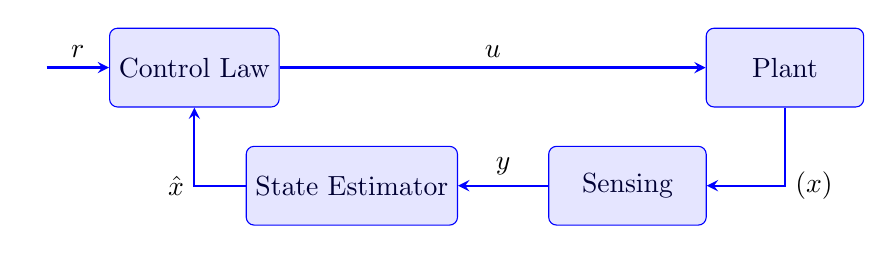
\begin{tikzpicture}[node distance=1.5cm]
    \node (in) [eNode] {};
    \node (control) [recNodeB, right of=in, xshift=0.5cm] {Control Law};
    \node (sys) [recNodeB, right of=control, xshift=6cm] {Plant};
    \node (sensor) [recNodeB, below of=sys, xshift=-2cm] {Sensing};
    \node (estimator) [recNodeB, below of=control, xshift=2cm] {State Estimator};
    
    \draw [arrowB] (in) -- node[above] { $r$} (control);
    \draw [arrowB] (control) -- node[above] { $u$} (sys);
    \draw [arrowB] (sys) |- node[right] { ($x$)} (sensor);
    \draw [arrowB] (sensor) -- node[above] { $y$} (estimator);
    \draw [arrowB] (estimator) -| node[left] { $\hat{x}$} (control);
    \end{tikzpicture}
  }
\def\myPeriodTable{
  \begin{tabular}{|c c c|} 
      \hline
      Task & Period & Deadline \\ 
      \hline
      Check for obstacles & 10ms & 1.5ms \\ 
      %\hline
      Check GPS position & 10ms & 0.5ms \\
      Control Law & 2ms & 0ms \\
      \multicolumn{3}{|c|}{$\cdots$}\\
      \hline
  \end{tabular}
}
\def\tikzSensorGameBase{    
    \node[state,initial,p1](env1) at (6.44,2.24){$env_1$};
    \node[state,accepting,p0](s1) at (6.44,-0.98){$s_1$};
    \node[state,accepting,p0](s2) at (10.52,2.2){$s_2$};
    \node[state,p0,grayed](sink) at (17.04,2.18){$sink$};
    \node[state,accepting,p0](s3) at (14.04,-0.98){$s_3$};
    \node[state,p1,grayed](env3) at (14.02,2.18){$env_3$};
    \node[state,p1](env2) at (10.52,-1.0){$env_2$};
    \path[->]
    (env1) edge [bend left=10] node {$0 \leq$ \qq $\leq 1$} (s1)
    (env1) edge [bend left=10] node {$1 \leq$ \qq $\leq 2$} (s2)
    (s1) edge [bend left=10] node {\HH,\ \LL} (env1)
    (s2) edge [bend left=10] node {\HH} (env1)
    (s2) edge [bend right=10] node [left] {\LL} (env2)
    (s3) edge [bend left=10,grayed] node {\LLL} (env3)
    (env3) edge [grayed] node {$1 \leq$ \qqq $\leq 2$} (s2)
    (env3) edge [grayed] node {\qqq $ > 3$} (sink)
    (env3) edge [bend left=10,grayed] node {$2 \leq$ \qqq $\leq 3$} (s3)
    (env2) edge [] node {$0 \leq$ \qq $\leq 1$} (s1)
    (env2) edge [bend right=10] node [right] {$1 \leq$ \qq $\leq 2$} (s2)
    (env2) edge [] node {$2 \leq$ \qq $\leq 3$} (s3)
    ;
    \path[->,draw] (s3) --  node {\HH} ++(0,-1) -- ++(-9,0) -- ++(0,3) -- (env1);
}
\def\tikzSensorGame{		
    \begin{tikzpicture}[
    auto,
    initial text=,
    semithick,
    >=stealth,
    ,
    p0/.style={circle,fill=yellow,thick},p1/.style={rectangle,fill=green,thick}
    ,grayed/.style={} %{fill=white, draw=lightgray,text=lightgray}
    ]
    \def\qqq{\qq}
    \def\LLL{\LL}
    \tikzSensorGameBase
    \end{tikzpicture}
}
\def\tikzSensorGameStrategy{		
    \begin{tikzpicture}[
    auto,
    initial text=,
    semithick,
    >=stealth,
    ,
    p0/.style={circle,fill=yellow,thick},p1/.style={rectangle,fill=green,thick}
    ,grayed/.style={fill=white, draw=lightgray,text=lightgray}
    ]
    \def\qqq{q}
    \def\LLL{L}
    \tikzSensorGameBase
    \end{tikzpicture}
}
\newcommand\tikzSensorGameMark[1]{		
    \begin{tikzpicture}[
    auto,
    initial text=,
    semithick,
    >=stealth,
    ,
    p0/.style={circle,fill=yellow,thick},p1/.style={rectangle,fill=green,thick}
    ,grayed/.style={} %{fill=white, draw=lightgray,text=lightgray}
    ]
    \def\qqq{\qq}
    \def\LLL{\LL}
    \tikzSensorGameBase
    \draw [ red, fill=blue!50] (#1) [yshift=0.4cm]  circle (0.4);
    \end{tikzpicture}
}
    
\frame{ %Example
  \frametitle{Example}
  \framesubtitle{A component that ``plays'' a game with its environment}
  \begin{center}
      \scalebox{0.8}{
          \tikzSensorGame
        }
  \end{center}
  \begin{block}{}
      \begin{itemize}
          \item A sensor with two modes: \HH igh quality, \LL ow quality.
          \item After \HH, the estimation quality (\qq) is best, after \LL it may degrade.

        \end{itemize}
  \end{block}
}
\frame{ %Example
    \frametitle{Example}
    \framesubtitle{A solution of the game}
    \begin{center}
        \scalebox{0.8}{
            \tikzSensorGameStrategy
        }
    \end{center}
    \begin{block}{}
        \begin{itemize}
            \item We must not schedule \HH\ when in $s_3$
        \end{itemize}
    \end{block}
}
\frame{ %Example
    \frametitle{Example}
    \framesubtitle{Simultaneous Games (composition)}
    \begin{columns}
        \begin{column}{0.6\textwidth}
            \scalebox{0.5}{
                \only<1>{\tikzSensorGameMark{env1}
                }\only<2>{\tikzSensorGameMark{s1}
                }\only<3>{\tikzSensorGameMark{env1}
                }\only<4>{\tikzSensorGameMark{s2}
                }\only<5>{\tikzSensorGameMark{env1}
                }\only<6>{\tikzSensorGameMark{s1}
                }\only<7>{\tikzSensorGameMark{env1}
                }\only<8>{\tikzSensorGameMark{s2}
                }\only<9>{\tikzSensorGameMark{env2}
                }\only<10>{\tikzSensorGameMark{s3}
                }\only<11->{\tikzSensorGameMark{env1}}
            }
            \\ ~ \\
            \scalebox{0.5}{
                \only<1>{\tikzSensorGameMark{env1}
                }\only<2>{\tikzSensorGameMark{s1}
                }\only<3>{\tikzSensorGameMark{env1}
                }\only<4>{\tikzSensorGameMark{s1}
                }\only<5>{\tikzSensorGameMark{env1}
                }\only<6>{\tikzSensorGameMark{s2}
                }\only<7>{\tikzSensorGameMark{env1}
                }\only<8>{\tikzSensorGameMark{s2}
                }\only<9>{\tikzSensorGameMark{env2}
                }\only<10>{\tikzSensorGameMark{s3}
                }\only<11->{\tikzSensorGameMark{env3}}
            }
        \end{column}
        
        { \small
        \begin{column}{0.45\textwidth}
            \begin{block}{}<12->
                We cannot allow both components to be on $env_{2}$
            \end{block}
            \begin{block}{}<13->
                If both components are at $s_2$, at least one \HH\ must be scheduled
            \end{block}
            \begin{block}{}<14>
                Adding a third component makes the system \textcolor{red}{unschedulable!}
            \end{block}
        \end{column}
        }
    \end{columns}
    \begin{block}{}
        Only one \HH\ per slot allowed
    \end{block}
}

\subsection[Architecture]{Component-based Architecture}

\def\tikzArch{
    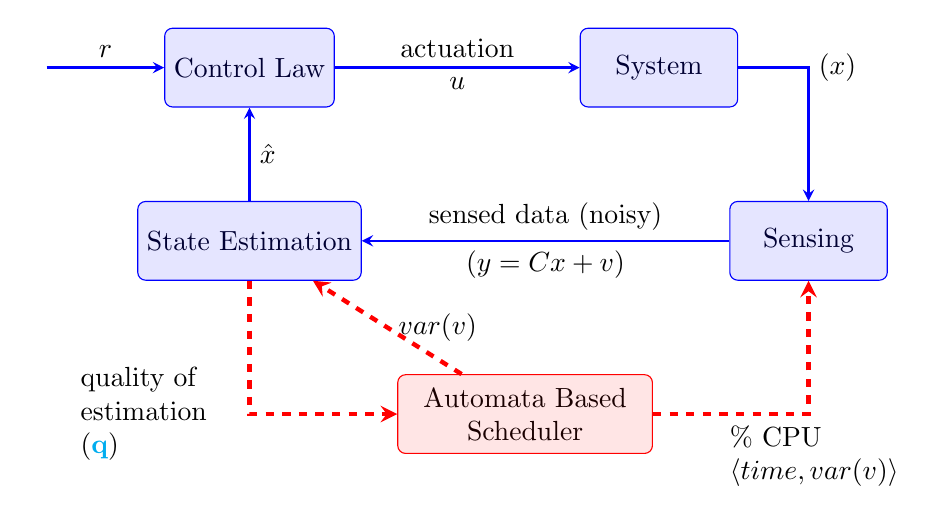
\begin{tikzpicture}[node distance=1.2cm]
    \node (in) [eNode] {};
    \node (control) [recNodeB, right of=in, xshift=1.5cm] {Control Law};
    \node (sys) [recNodeB, right of=control, xshift=4cm] {System};
    \node (sensor) [recNodeB, below of=sys, xshift=1.9cm, yshift=-1cm] {Sensing};
    \node (estimator) [recNodeB, below of=control, yshift=-1cm] {State Estimation};
    \node (sched) [recNodeG, below of=estimator, yshift=-1cm, xshift=3.5cm, text width=3cm] {Automata Based Scheduler};
    
    \draw [arrowB] (in) -- node[above] {$r$} (control);
    \draw [arrowB] (control) -- node[above] {actuation} node[below] {$u$} (sys);
    \draw [arrowB] (sys) -| node[right,text width=1cm] {($x$)} (sensor);
    \draw [arrowB] (sensor) -- node[above] {sensed data (noisy)} node[below] {$(y = Cx +v$)} (estimator);
    \draw [arrowB] (estimator) -- node[left,text width=2cm] {} node[right] {$\hat{x}$} (control);
    
    \draw [arrowG] (estimator) |- node[left,text width=2cm] {quality of estimation (\qq)} (sched);
    
    \draw [arrowG] (sched) -| node[below,text width=2cm] { \% CPU $\langle time,var(v) \rangle$} (sensor);
    %\draw [arrowG] (sched) -| node[right] {$\langle time,var(v) \rangle$} (sensor);
    
    \draw [arrowG] (sched) --  node[right] {$var(v)$} (estimator);
    
    \end{tikzpicture}
}

\frame{
    \frametitle{The Proposed Architecture}
    \framesubtitle{The scheduler is part of the control loop}
    \begin{center}
            \scalebox{0.9}{
                \tikzArch
            }
    \end{center} 
}
\subsection[Component]{Component definition}
%TODO \subsection[Component Definition]{Sub-Summery: Component Definition}
\frame{
    \frametitle{A Component in the System}
    \begin{center}
        \begin{columns}
            \begin{column}{0.5\textwidth}
                \scalebox{0.4}{
                    \tikzSensorGame
                }
            \end{column}
            \begin{column}{0.2\textwidth}
                \begin{block}{}
                    \tiny
                    High () \{\\
                    ~~~~ ...\\
                    \}\\
                    Low () \{\\
                    ~~~~ ...\\
                    \}
                \end{block}
            \end{column}
        \end{columns}
    \end{center}
    \begin{block}{Scheduling \buchi Game}
        \begin{itemize}
            \item \textbf{Alternating turns}
            \item Scheduler alphabet is $\Sigma_{schd} = 2^T$ {\small (in the example $T=\{H, L\} $)}
            \item Environment alphabet is $\Sigma_{env} = \mathbb{R}^n$ {\footnotesize (\textit{scheduler feedback variables})}
            \item There is an transition for any \textbf{possible} environmental outcome 
            \item The \textbf{scheduler feedback variables} can be any environment-depended value
            \item Environment player plays first
        \end{itemize}
    \end{block}
}
\frame{
    \frametitle{The Proposed Architecture}
    \framesubtitle{Automata-Based Specification Interface}
    %\todoil{maybe add a word about RTcomposer and GameComposer}\\
    \begin{block}{Automata advantages}
        \begin{itemize}
            \item \textbf{Lite:} minimal resource consumption at run-time
            \item \textbf{Expressive}
            \item \textbf{Composable}
            \item \textbf{Automata theory:} allows for tools such as \emph{GOAL}
        \end{itemize}
    \end{block}
    \hfill
    \begin{center}
        
\includegraphics[width=40mm]{GOAL}\\
        Graphical tool for Omega-Automata and Logics
    \end{center}
}

    
\section[Kalman Filter]{Simulation with Kalman}

\frame{
    \frametitle{Simulation}
    
    \begin{block}{} %{Resource utilization with Kalman filter}
         Schedule sensing-tasks based on the estimation quality
    \end{block}
    \begin{center}
        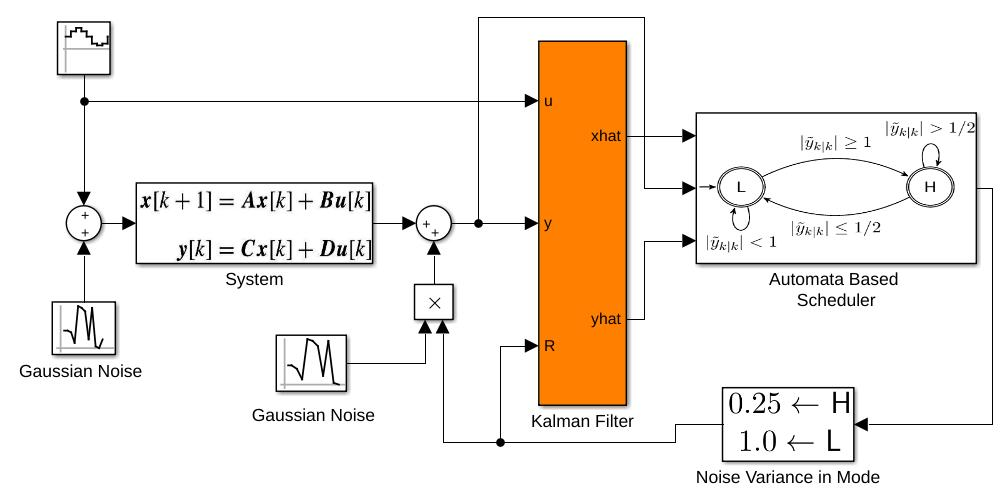
\includegraphics[width=90mm]{simulinkNew}
    \end{center}
    \only<2->{
        \begin{center}
            \scalebox{1}{
                \begin{tabular}{ |  l  | c | c | c | }
                    \hline
                    &  High & Low & Aut. Based \\ 
                    \hline %\hline
                    \%CPU  & 85 & 10  & 46 \\ 
                    \hline
                    mean of $|x -\hat{x}|$ & 0.97 & 1.24 & 1.08 \\ \hline
                \end{tabular}
            }
        \end{center}
    }
}
\frame{
    \frametitle{Integration with Kalman filter}
    \begin{center}
        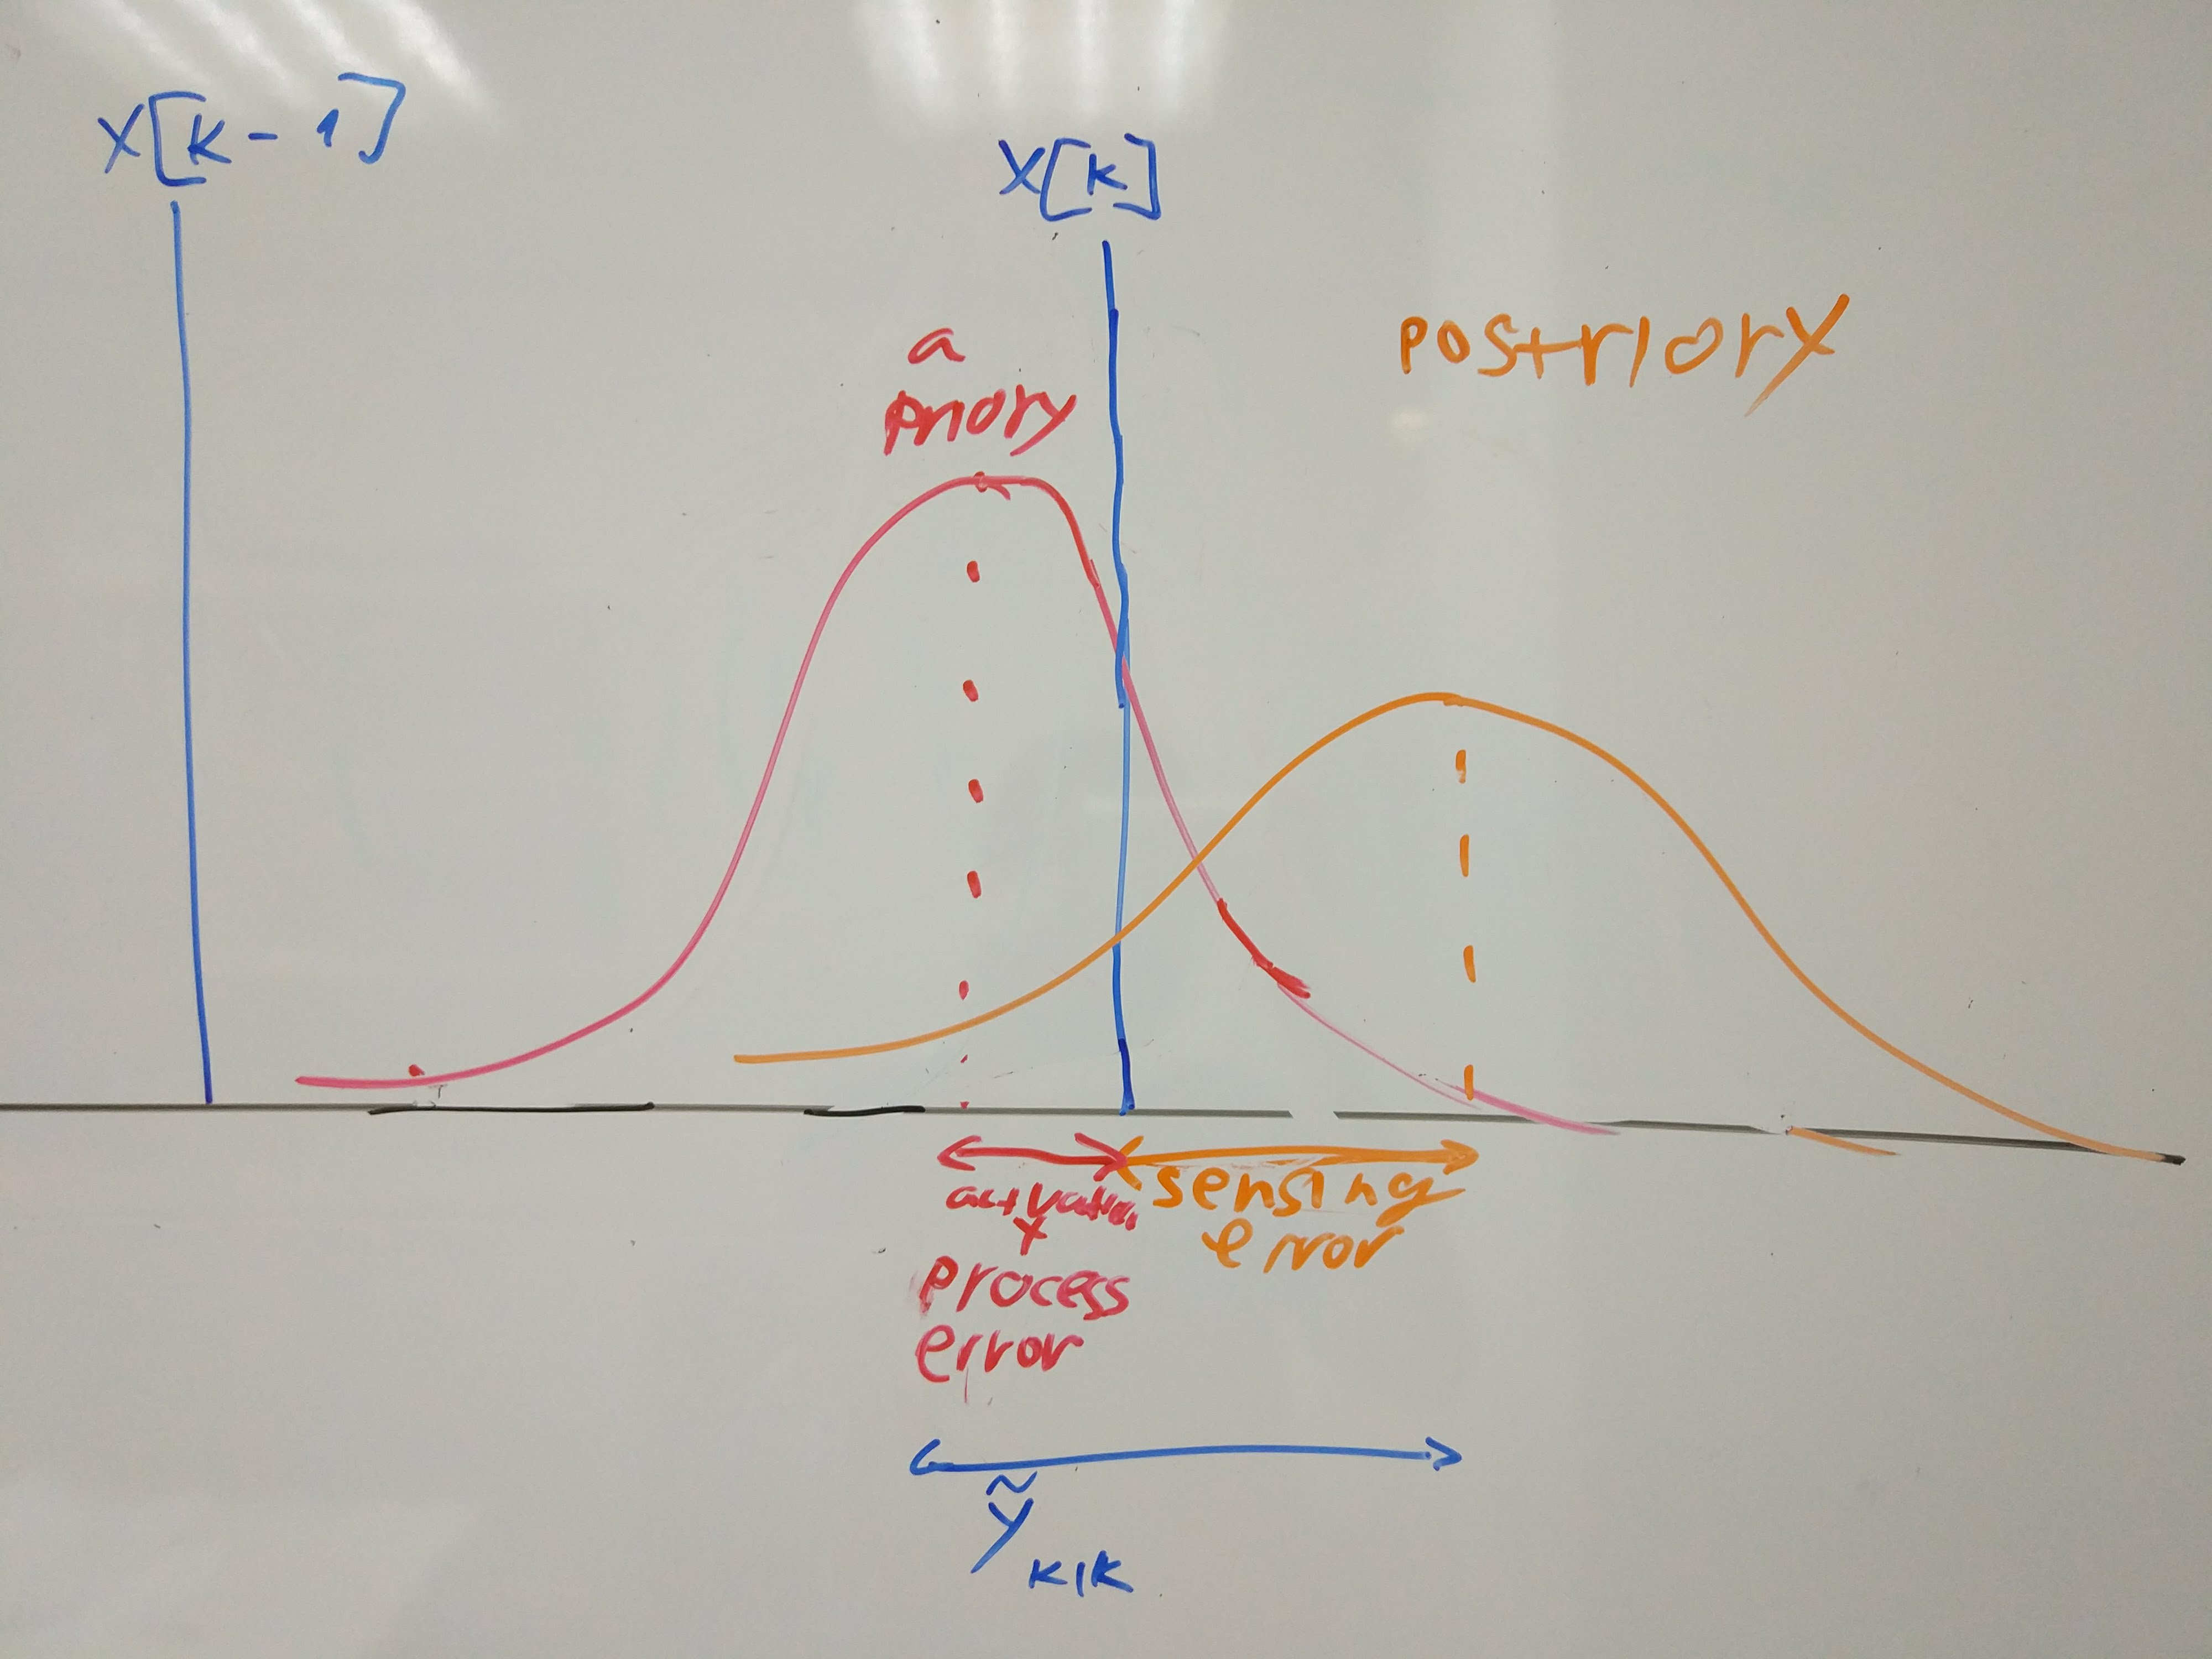
\includegraphics[width=30mm]{kalmanGraph}
    \end{center}
    \begin{block}{}
        \begin{itemize}
            \item Process \& actuation noise affect the \textit{a-priory} estimation 
            \item Measurement error affect only the measurement
            \item The difference between them estimate the over-all errors
        \end{itemize}
    \end{block}
}

\section[Experiment]{Experiment with real-life case-study}
\subsection{Case study}
\frame{
    \frametitle{Mission Definition}
    %\todoil{Explain the window motivation}
    \begin{center}
        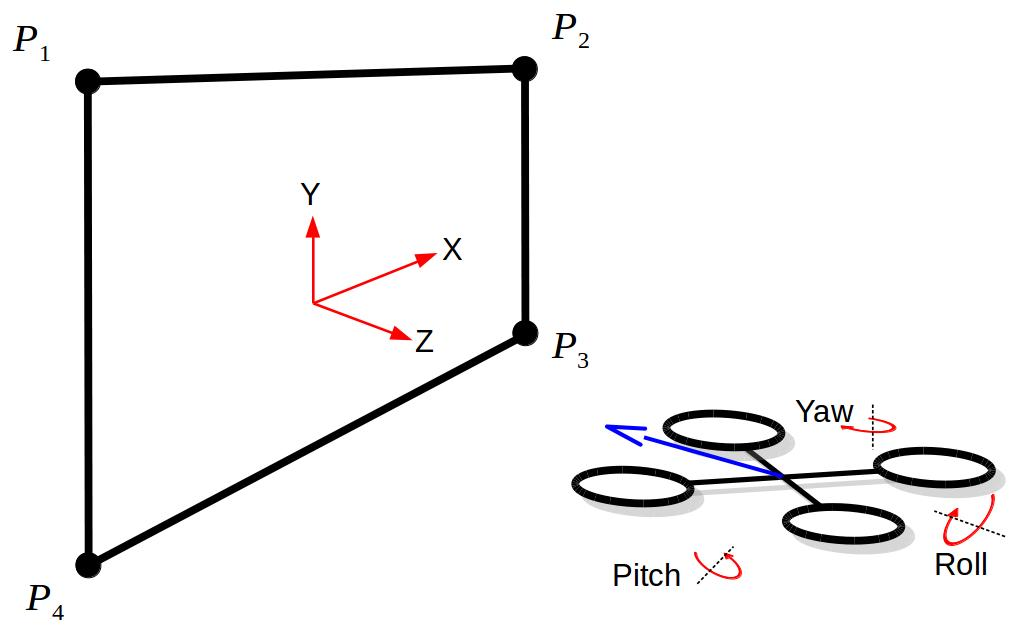
\includegraphics[width=100mm]{axis}
    \end{center}
}
\frame{
    \frametitle{Control Objectives}
    \begin{center}
        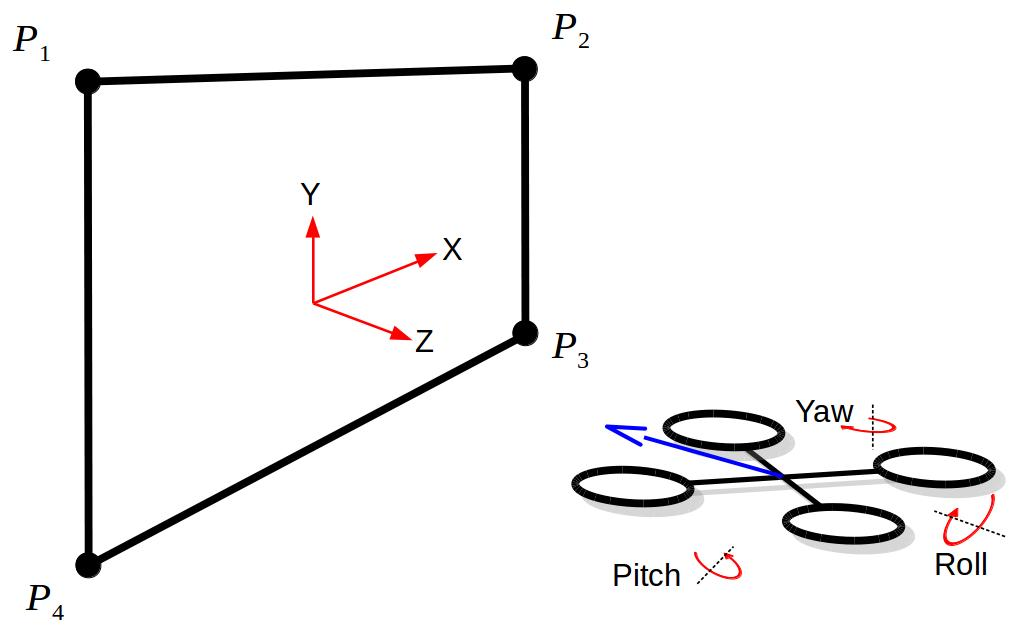
\includegraphics[width=70mm]{axis}
    \end{center}
    \begin{block}{ Control \& Scheduling Objectives }
        \begin{itemize}
            \item Minimize deviation in the $x$ axis
            \item Minimize CPU usage of the image processing task
        \end{itemize}
    \end{block}
}
\frame{
    \frametitle{Controller Design}
    \begin{center}
        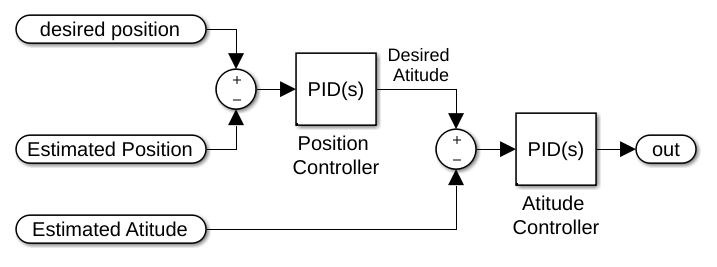
\includegraphics[width=90mm]{two_level_controller}
    \end{center}
    \begin{block}{ Attitude and position controller }
        \begin{itemize}
            \item The \textcolor{magenta}{\textbf{vision}} component estimate the position
            \item Position controller output a desired angle (proportional to acceleration)
            \item We used a standard PID controllers
        \end{itemize}
    \end{block}
}

\subsection{Vision Component}
\frame{
    \frametitle{Vision Component}
    \begin{center}
        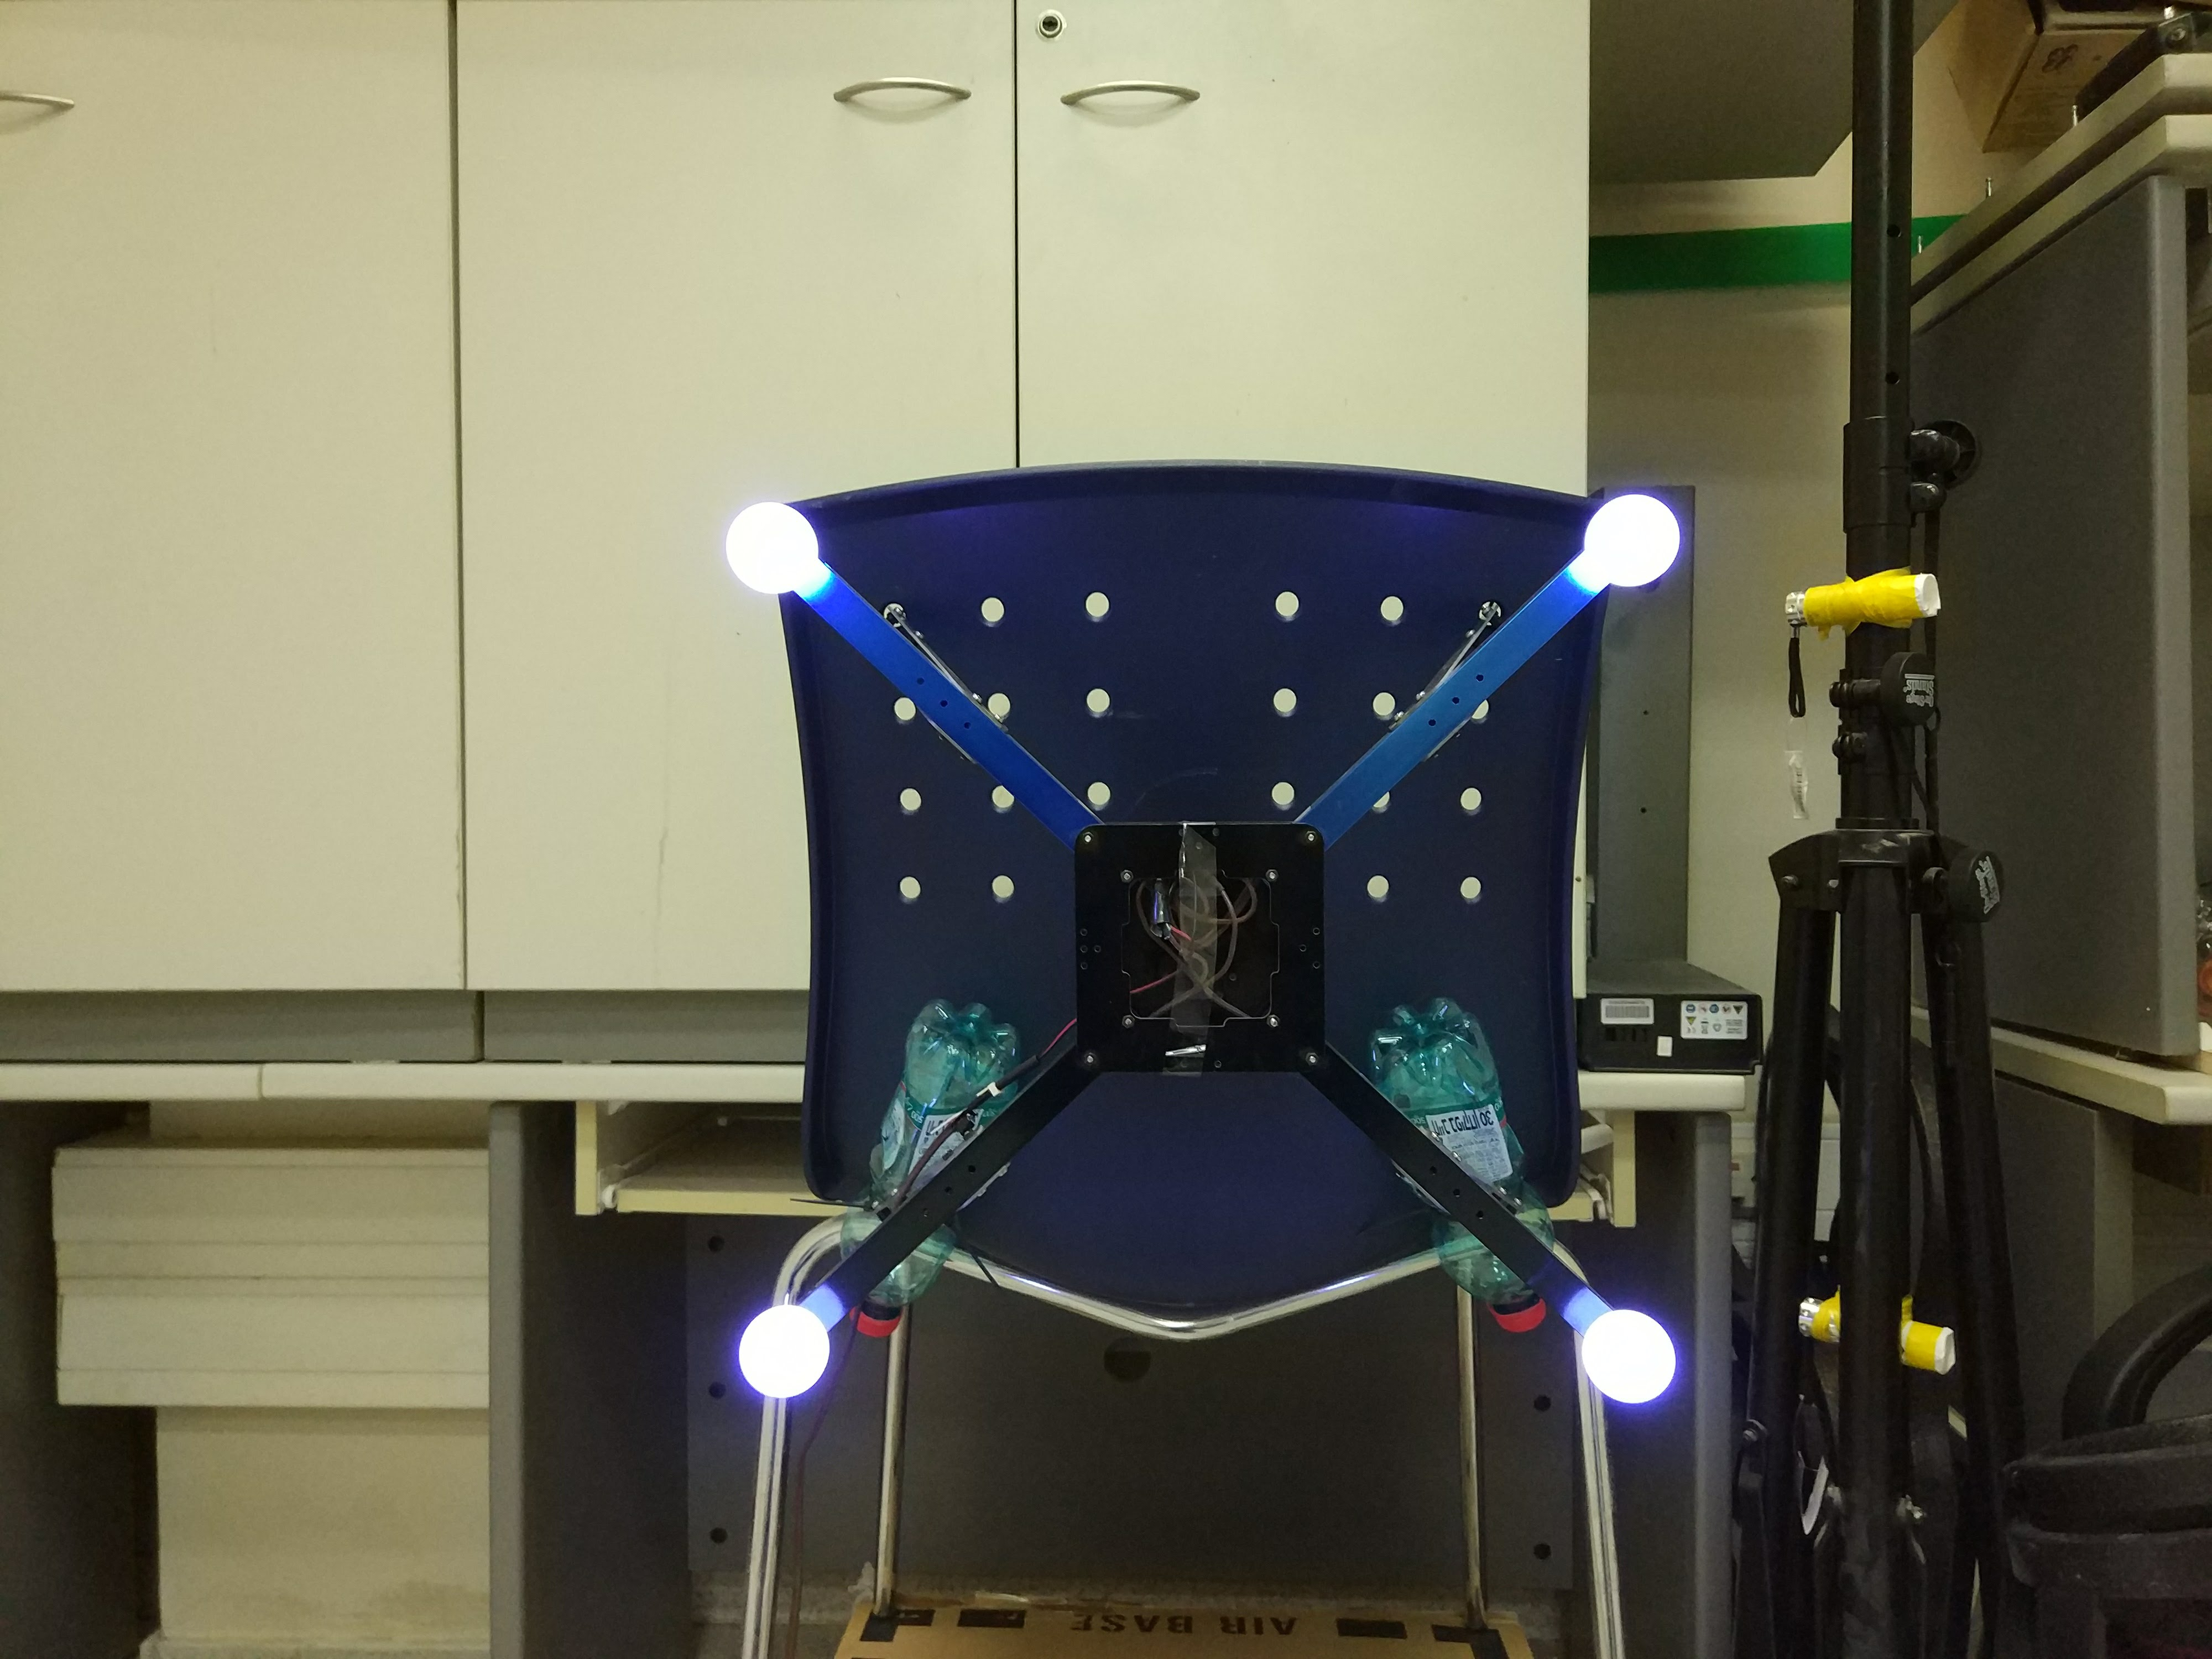
\includegraphics[width=60mm]{windowFront}
    \end{center}
    \begin{block}{ Image Processing Algorithm }
        \begin{enumerate}
            \item Find the window corners (brute force search)
            \item Calculate the drone position
        \end{enumerate}
    \end{block}
}
\frame{ % $V_d$
    \frametitle{Calculate the Drone Position}
    \framesubtitle{Vertical Difference}
    \begin{center}
        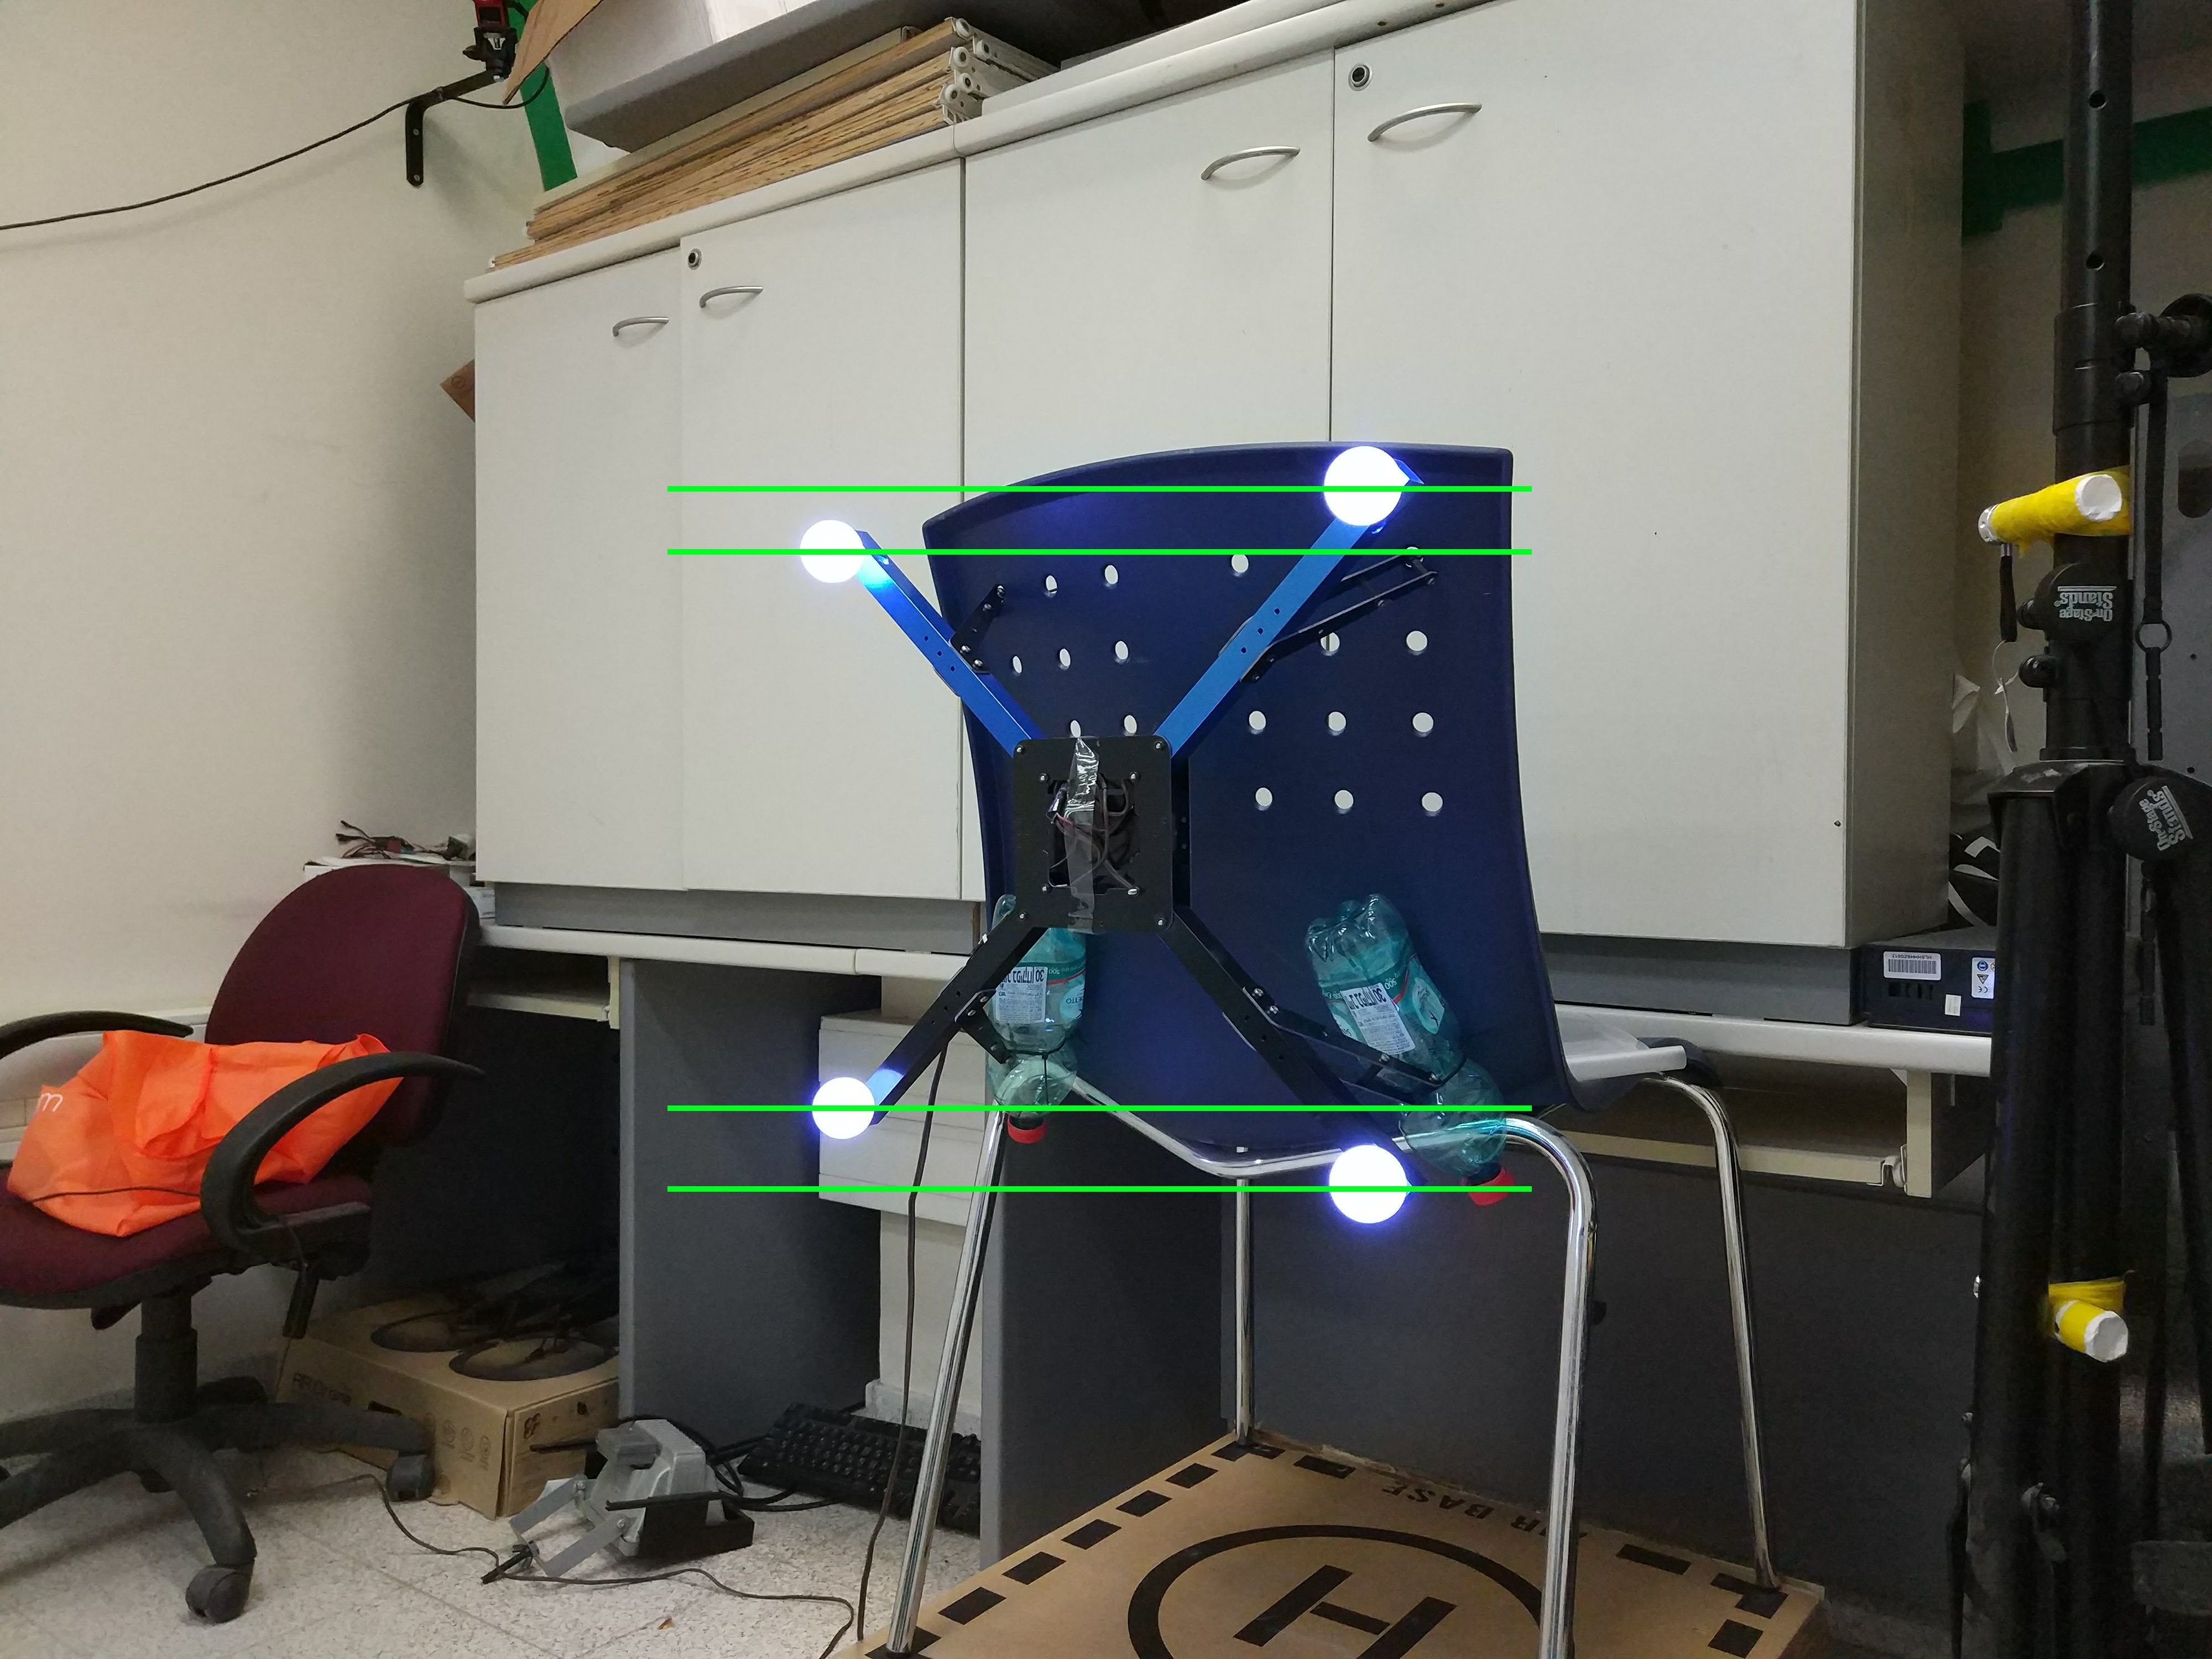
\includegraphics[width=60mm]{windowVd}
    \end{center}
    \begin{block}{ }
        \centering {\Large $V_d = \frac{((y_1-y_4)-(y_2-y_3))}{((y_1-y_4)+(y_2-y_3))}$}
        \\~\\
        {\Large $sz =$} {\small ${((y_1-y_4)-(y_2-y_3))} + {((y_1-y_4)+(y_2-y_3))}$}
    \end{block}
}
\frame{ % $S_x$
    \frametitle{Calculate the Drone Position}
    \framesubtitle{Center of Mass}
    \begin{center}
        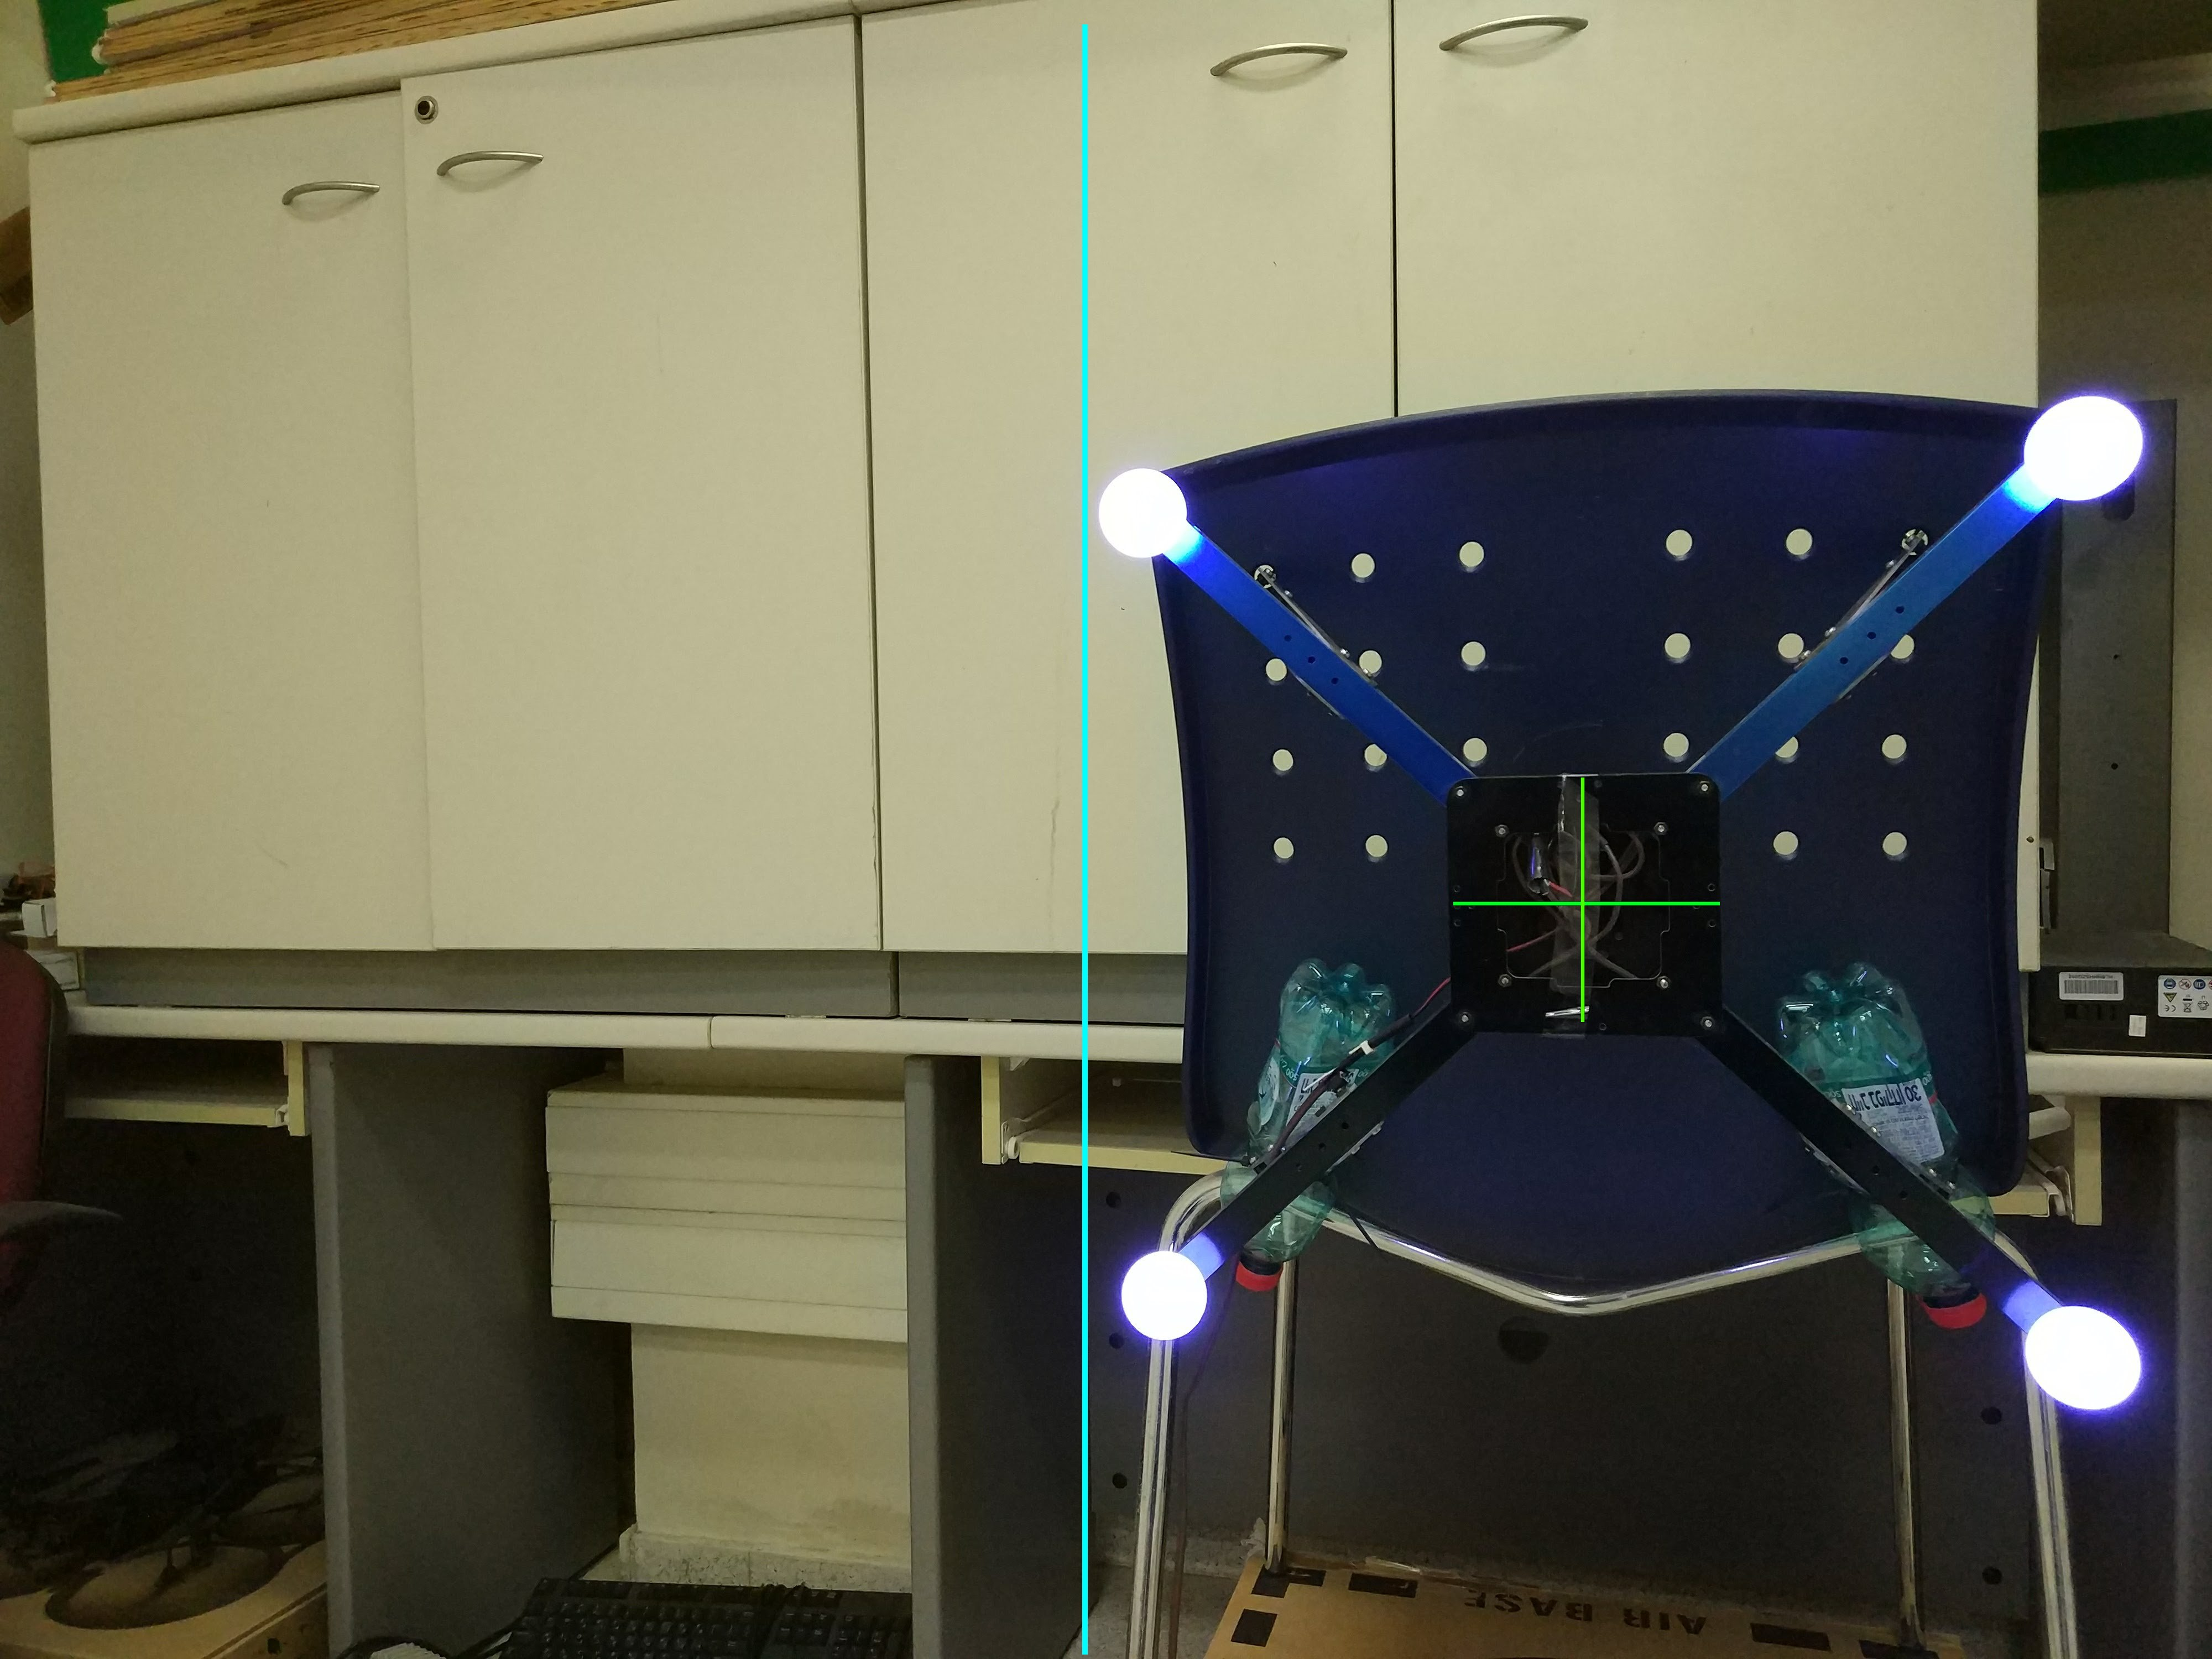
\includegraphics[width=60mm]{windowYaw}
    \end{center}
    \begin{block}{ }
        \centering \Large $S_x = \frac{x_1 + x_2 + x_3 + x_4}{4}$
    \end{block}
}
\frame{ % $x = l V_d$
    \frametitle{Calculate the Drone Position}
    \framesubtitle{Aproximate $x$ Position}
    \begin{center}
        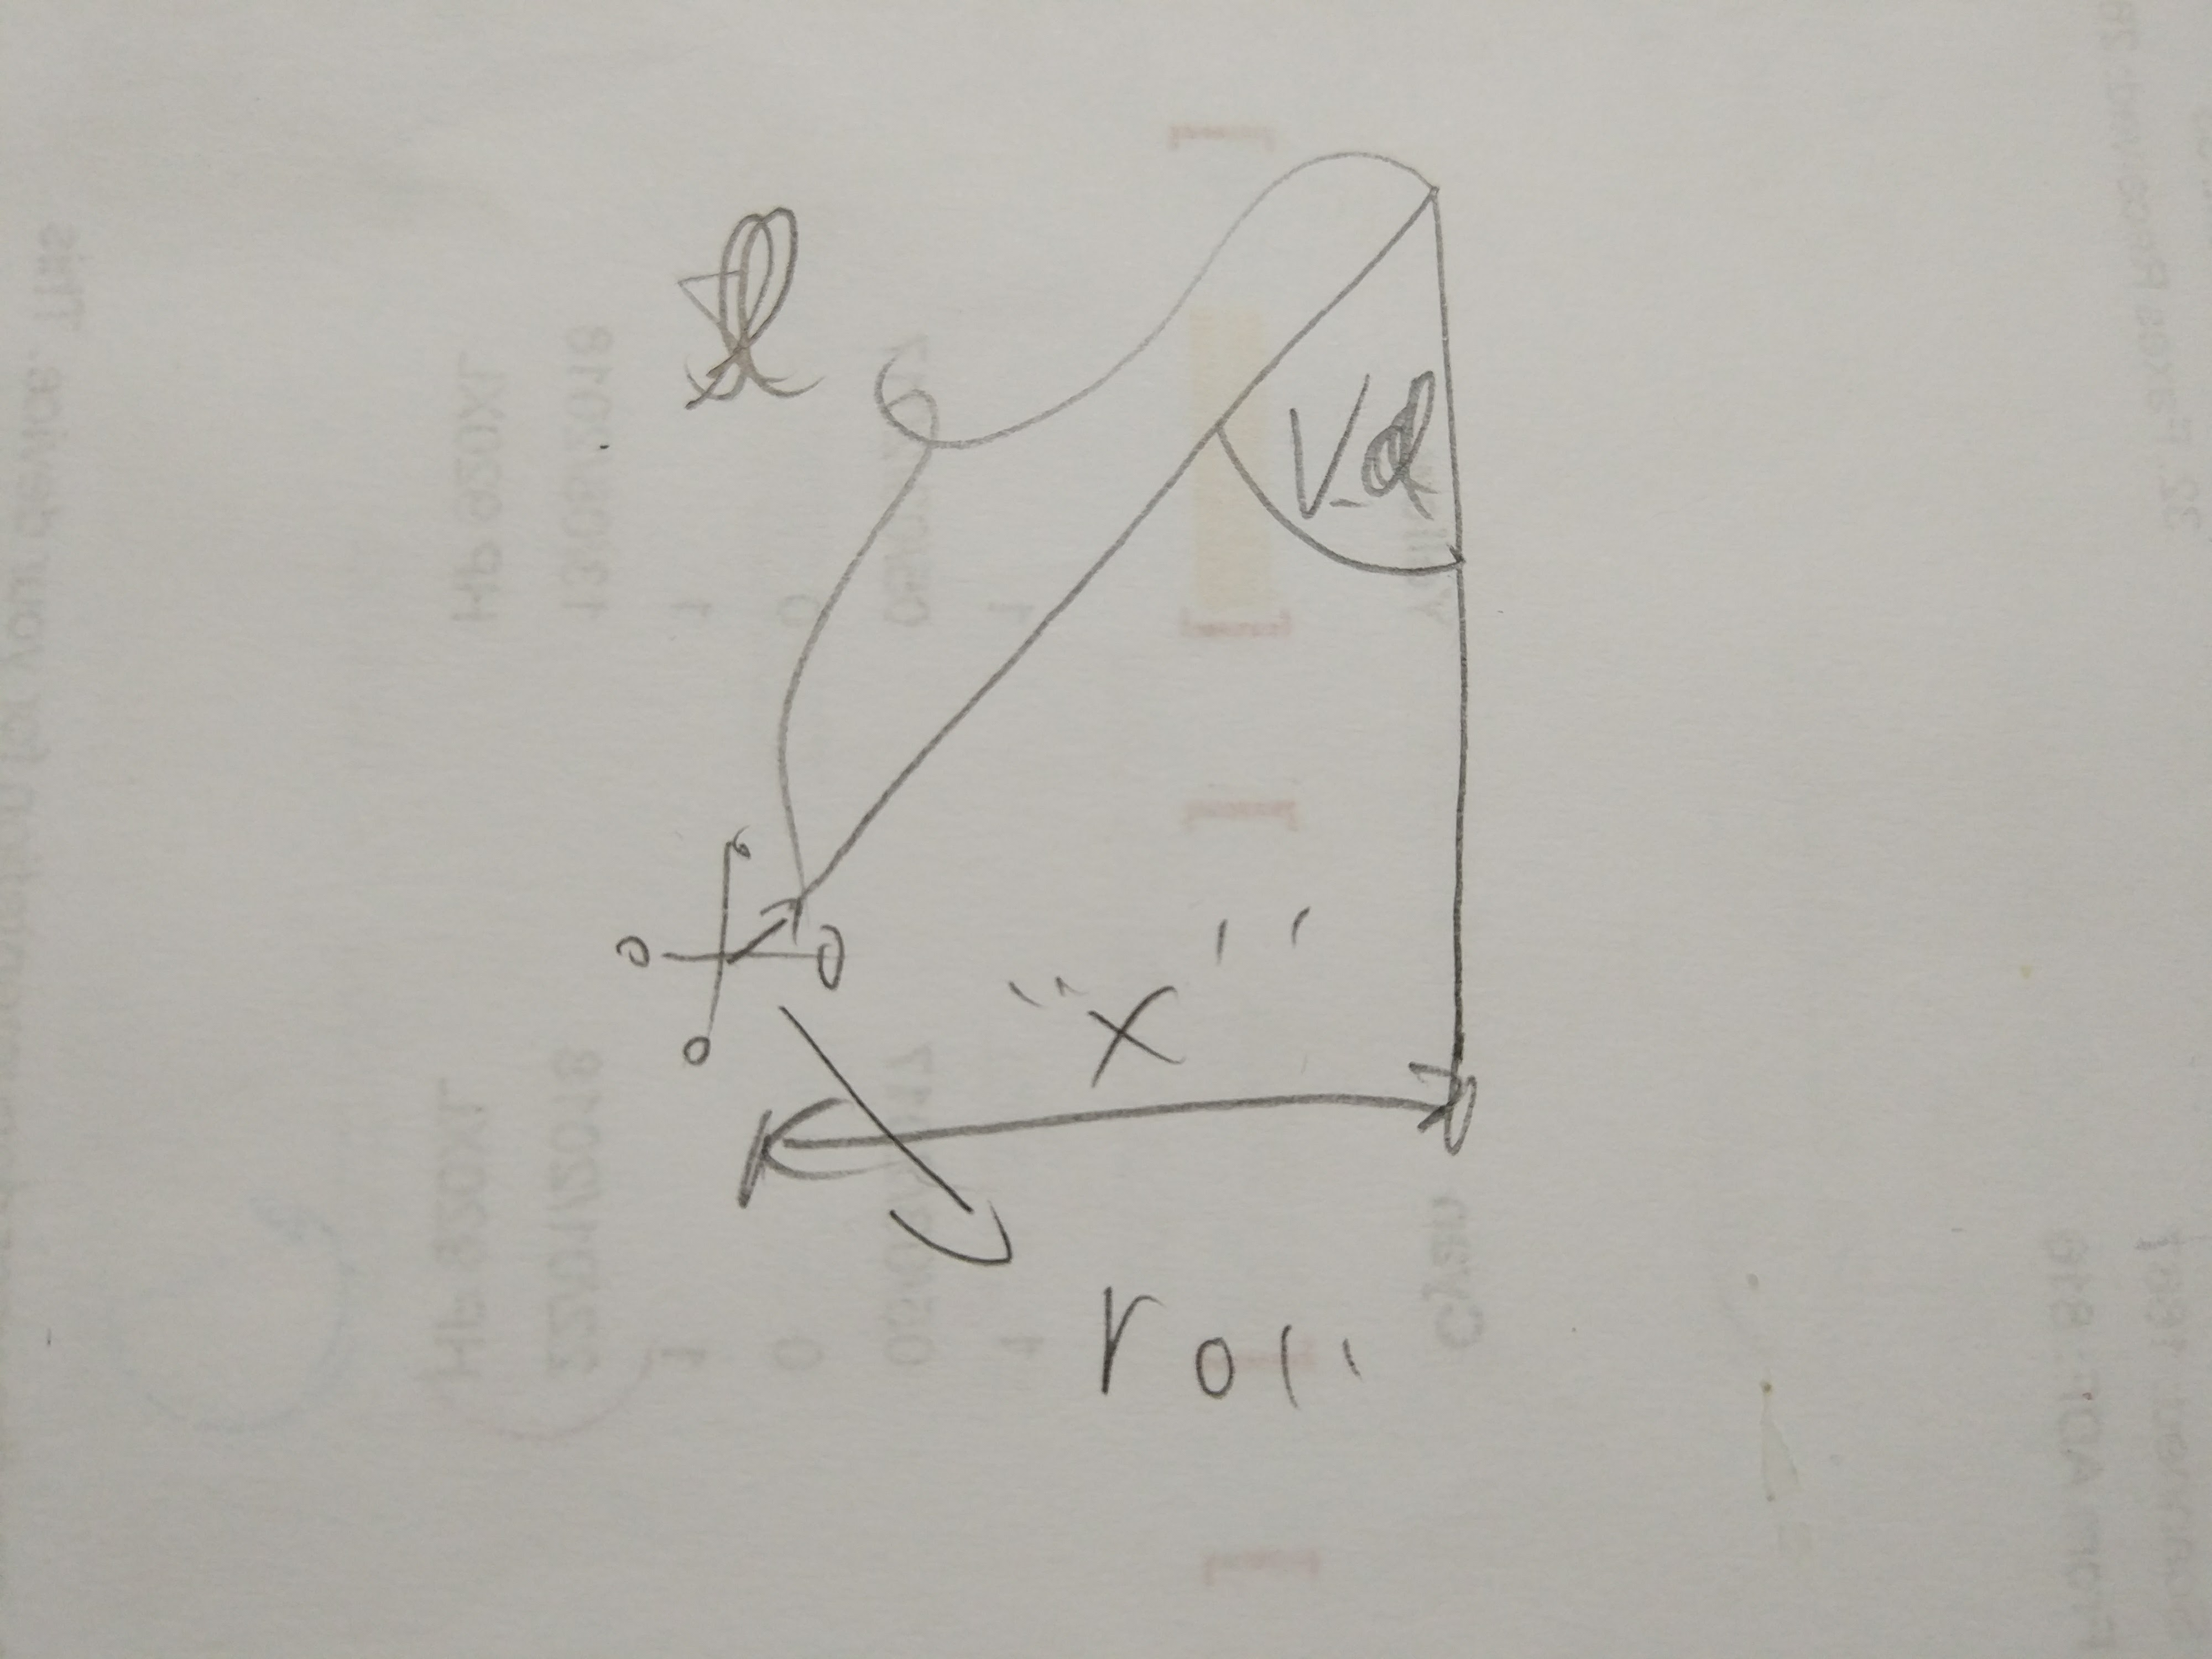
\includegraphics[width=50mm]{vd-geometry}
    \end{center}
    \begin{block}{ }
        $x = l \cdot \sin(V_d) \approx l \cdot V_d$
    \end{block}
}

\subsection[Filtering]{Simplifying the Kalman Filter with Complementary Filter}
\frame{
    \frametitle{The Filter}
    \begin{block}{ Limitations of Kalman filter }
        \begin{itemize}
            \item The system is  not linear
            \item The process and actuation noises distribution are unknown and unstable
            \item Kalman filter adds complexity in the code
        \end{itemize}
    \end{block}
    \begin{block}{ Filtering in two steps }
        \begin{enumerate}
            \item \textcolor{purple}{Predicts} - with a linearized model
            \item \textcolor{blue}{Update} - with the vision and other sensors
        \end{enumerate}
    \end{block}
}
\frame{
    \frametitle{The Linearized Model}
    \begin{columns}
        \begin{column}{5cm}
            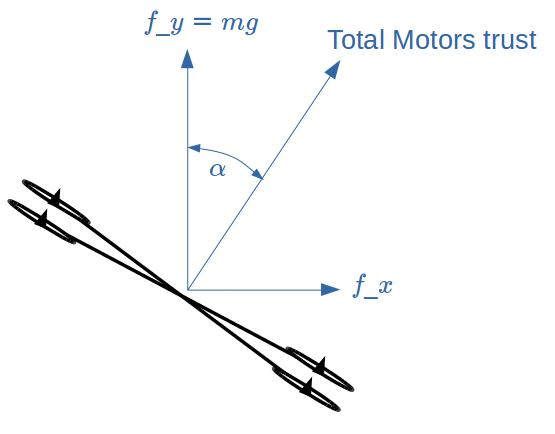
\includegraphics[width=50mm]{acceleration_static_diagram}
        \end{column}
        \begin{column}{5cm}
            \begin{block}{ }
                \[ A = 
                \left( \begin{array}{ccc}
                1 & dt & 0 \\
                0 & 1 & dt \\
                0 & 0 & 0 \end{array} \right)\] 
                
                \[ B = 
                \left( \begin{array}{c}
                0 \\
                0 \\
                g \end{array} \right)\] 
            \end{block}
        \end{column}
    \end{columns}
    \begin{block}{ Basic equations of motion on $x$ axis}
        \begin{itemize}
            \item \textbf{Position}: $\bar{r}_x[k+1] = r_x[k] + dt \cdot v_x[k]$
            \item \textbf{Velocity}: $\bar{v}_x[k+1] = v_x[k] + dt \cdot a_x[k]$
            \item \textbf{Acceleration}: $\bar{a}_x[k+1] = \Sigma F_x / m \approx roll \cdot g $
        \end{itemize}
    \end{block}
}
\frame{
    \frametitle{The Measurement vector}
    \begin{columns}
        \begin{column}{5cm}
            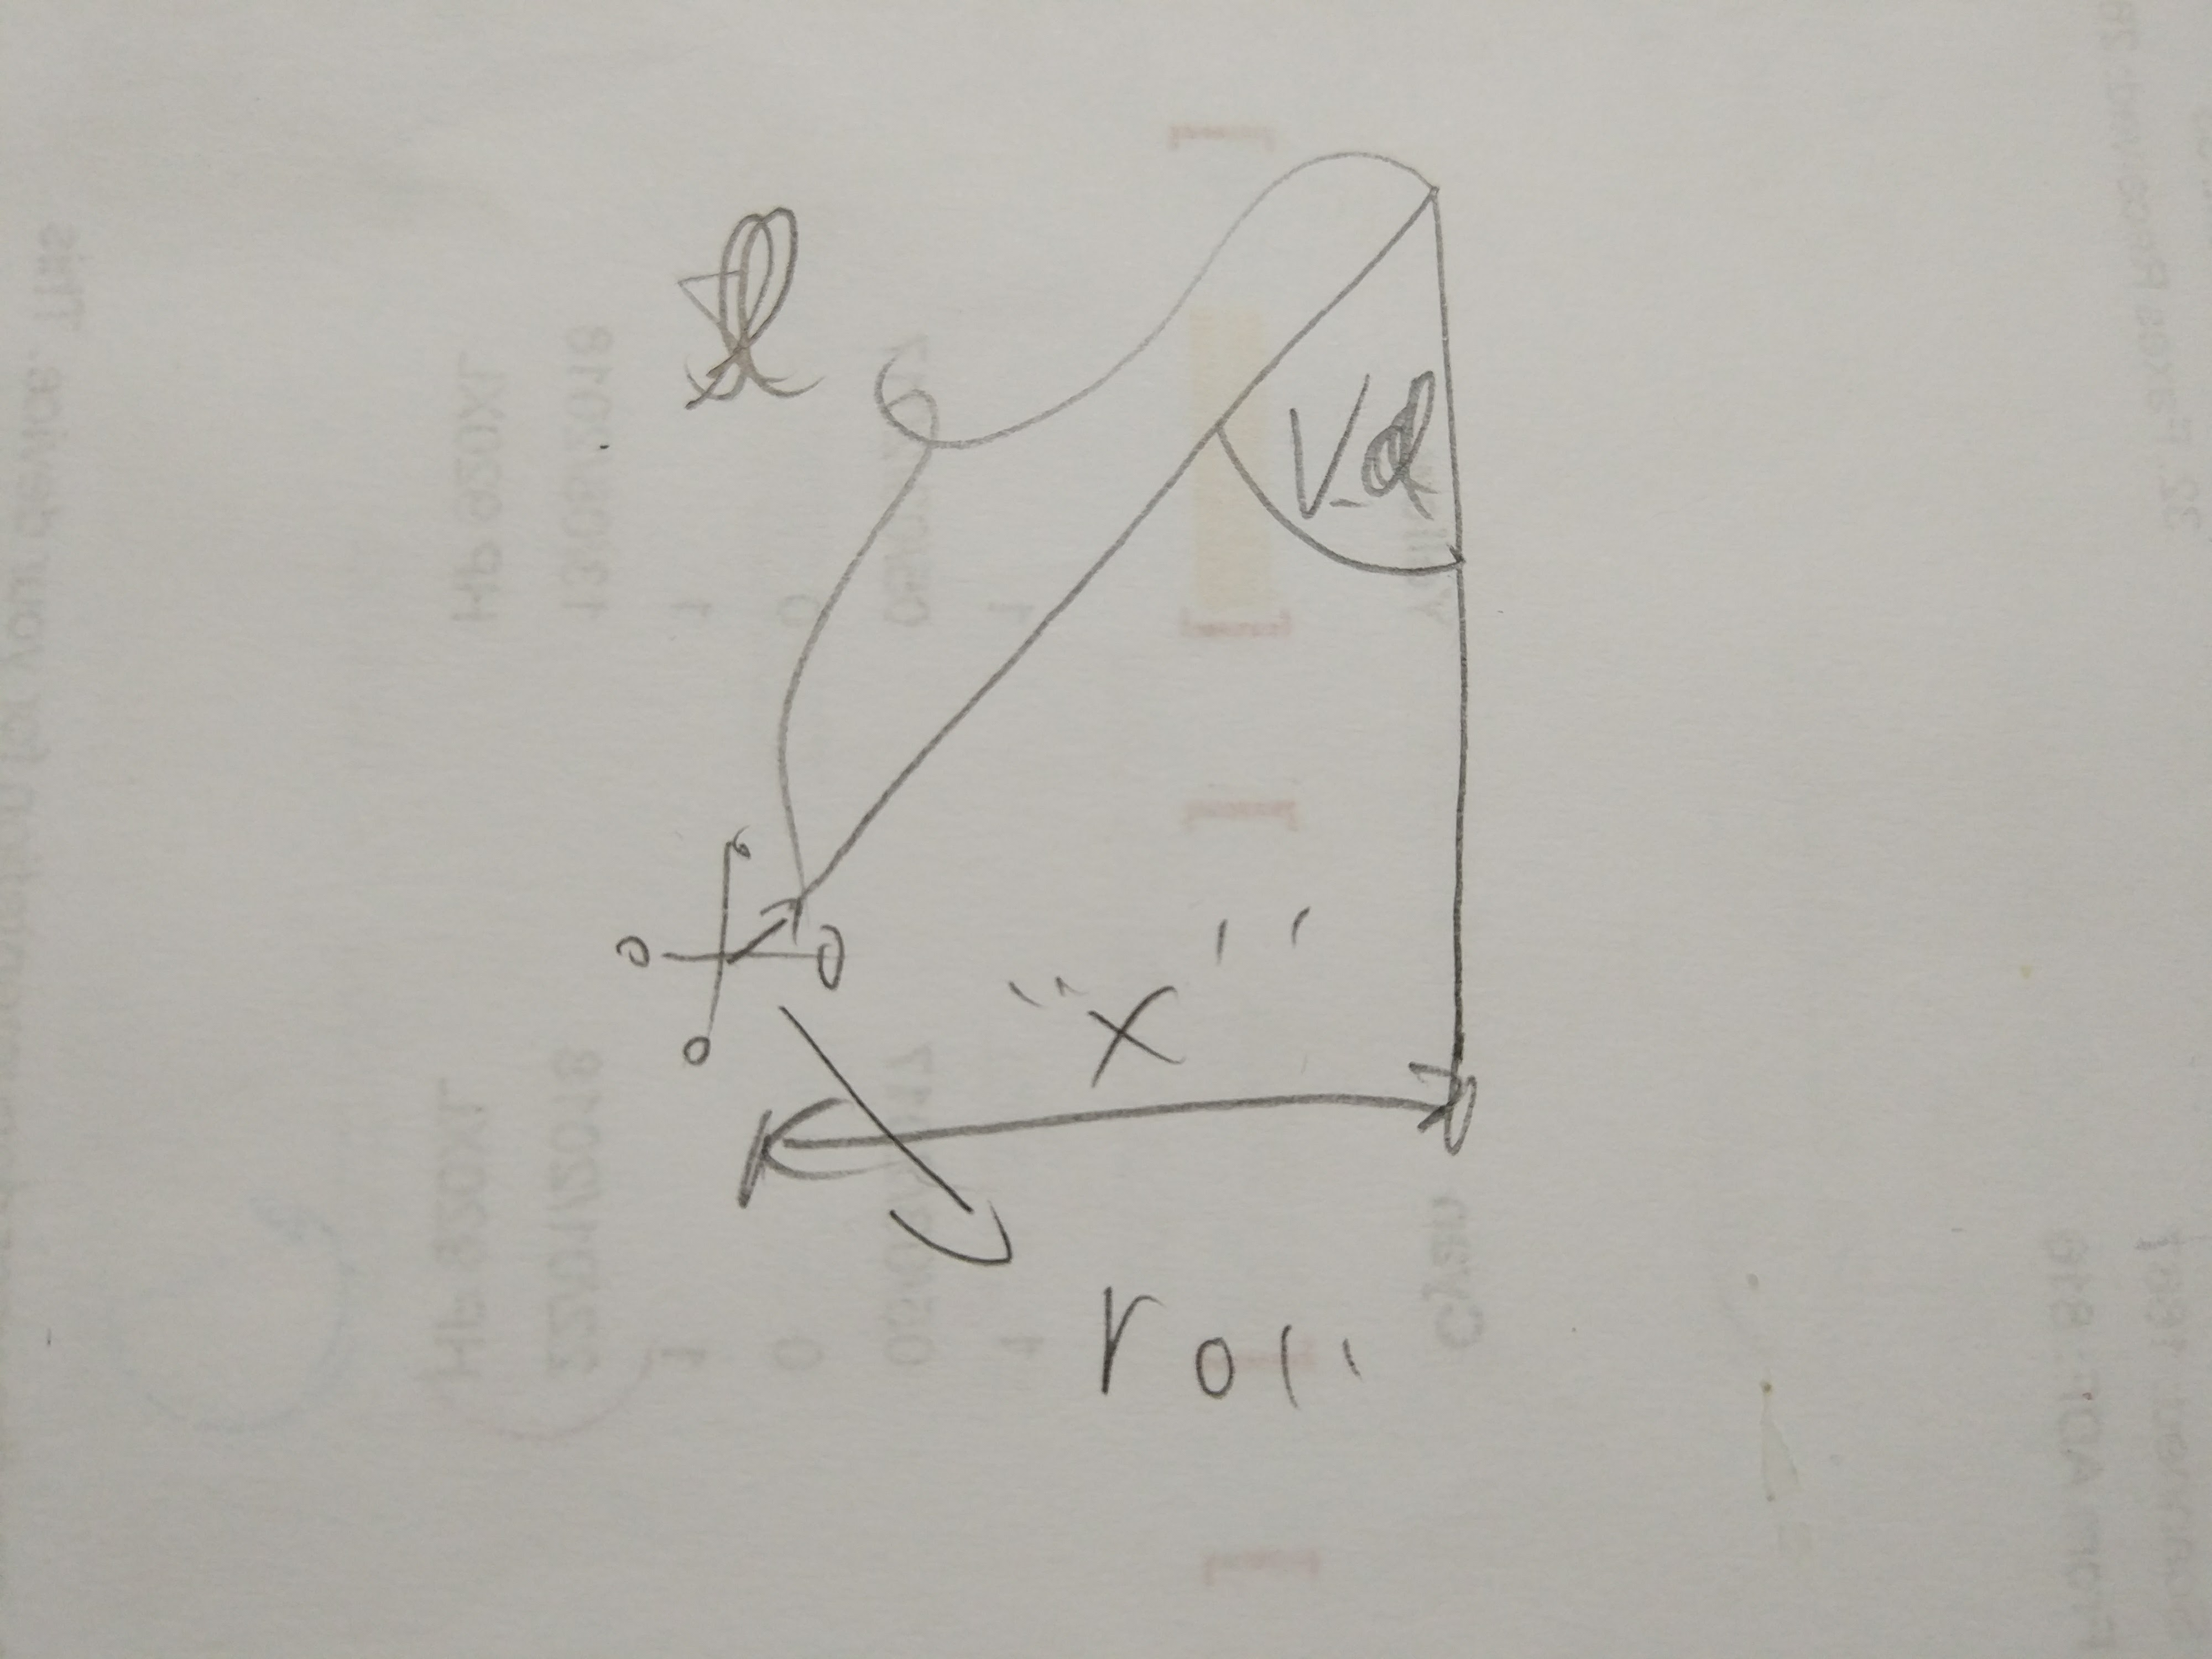
\includegraphics[width=40mm]{vd-geometry}
        \end{column}
        \begin{column}{5cm}
            \begin{block}{ }
                \[ C = 
                \left( \begin{array}{ccc}
                1 & 0 & 0 \\
                0 & 1 & 0 \\
                0 & 0 & 1/g \end{array} \right)\] 
            \end{block}
        \end{column}
    \end{columns}
    \begin{block}{ Measurement vector}
        \begin{itemize}
            \item \textbf{Position}: from vision algorithm
            \item \textbf{Velocity}: $ \frac{\partial r_x}{\partial t}$
            \item \textbf{Acceleration}: roll angle from the AHRS of APM
        \end{itemize}
    \end{block}
}
\frame{
    \frametitle{The Update Step}
    \begin{block}{ }
        $ x[k] = K \cdot \bar{x}[k] + (1-K) \cdot C^{-1} \cdot y[k] $
    \end{block}
    \begin{block}{ }
        $ x_r = K_r \cdot \bar{x_r}[k] + (1-K_r) \cdot y_r[k] $\\
        $ x_v = K_v \cdot \bar{x_v}[k] + (1-K_v) \cdot y_v[k] $\\
        $ x_a = \bar{x_a}$
    \end{block}
    \begin{block}{ Overall noise estimation }
        $ \tilde{y}_{k|k} = \bar{x_r}[k] - y_r[k] $
    \end{block}
}

\subsection[Results]{Test and Results}
\def\tikzGPU{
    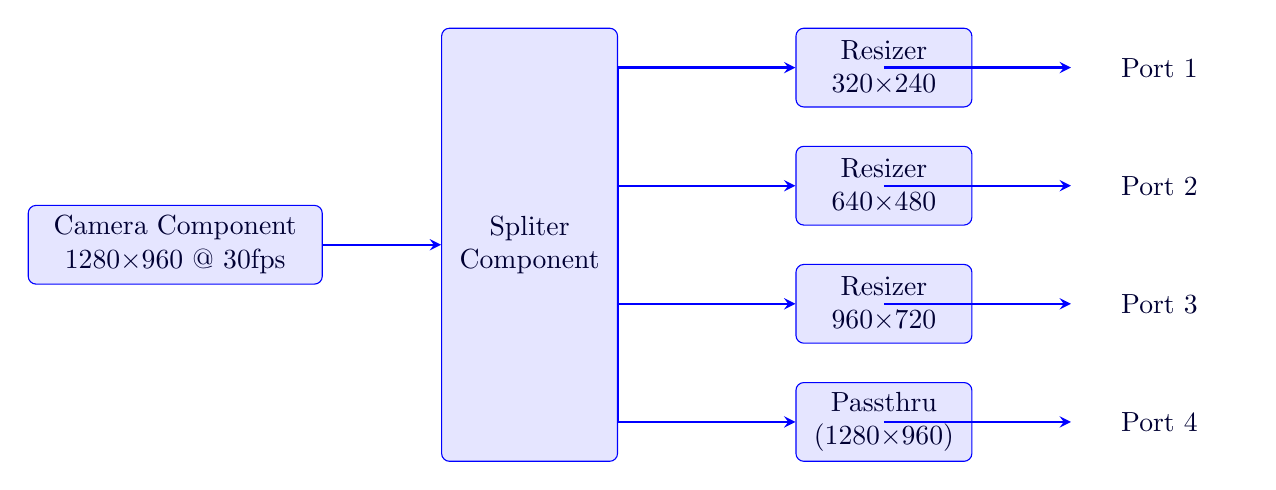
\begin{tikzpicture}[node distance=4.5cm]
    \node (cam) [recNodeB, text width=3.5cm] {Camera Component 1280$\times$960 @ 30fps};
    \node (sp) [recNodeB, text width=2cm, right of=cam, minimum height=5.5cm] {Spliter Component};
    \node (r1) [recNodeB, text width=2cm, right of=sp, yshift=2.25cm] {Resizer 320$\times$240 };
    \node (r2) [recNodeB, text width=2cm, right of=sp, yshift=0.75cm] {Resizer 640$\times$480};
    \node (r3) [recNodeB, text width=2cm, right of=sp, yshift=-0.75cm] {Resizer 960$\times$720};
    \node (r4) [recNodeB, text width=2cm, right of=sp, yshift=-2.25cm] {Passthru (1280$\times$960)};
    
    \draw [arrowB] (cam) -- node[above] {} (sp);
    \draw [arrowB] (sp.east) |- node[] {  } (r1.west);
    \draw [arrowB] (sp.east) |- node[] {  } (r2.west);
    \draw [arrowB] (sp.east) |- node[] {  } (r3.west);
    \draw [arrowB] (sp.east) |- node[] {  } (r4.west);
    
    \node (p1) [eNode, text width=2cm, right of=r1, xshift=-1cm] {Port 1};
    \node (p2) [eNode, text width=2cm, right of=r2, xshift=-1cm] {Port 2};
    \node (p3) [eNode, text width=2cm, right of=r3, xshift=-1cm] {Port 3};
    \node (p4) [eNode, text width=2cm, right of=r4, xshift=-1cm] {Port 4};
    
    \draw [arrowB] (r1) |- node[] {  } (p1);
    \draw [arrowB] (r2) |- node[] {  } (p2);
    \draw [arrowB] (r3) |- node[] {  } (p3);
    \draw [arrowB] (r4) |- node[] {  } (p4);
    \end{tikzpicture}
}
\def\AutoErr{
    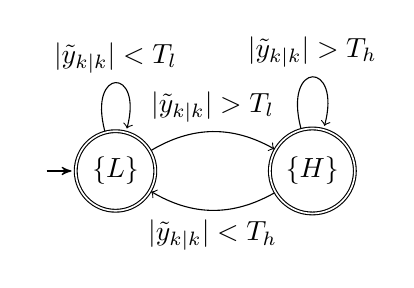
\begin{tikzpicture}[node distance=2.5cm,auto]
        \node (A) [state, accepting, initial] {$\{L\}$};
        \node (B) [state, accepting] [right of=A] {$\{H\}$};
        
        \path[->] (A) edge [loop above] node {$|\tilde{y}_{k|k}| < T_l$} (A);
        \path[->] (A) edge [bend left] node {$|\tilde{y}_{k|k}| > T_l$} (B);
        \path[->] (B) edge [bend left] node {$|\tilde{y}_{k|k}| < T_h$} (A);
        \path[->] (B) edge [loop above] node {$|\tilde{y}_{k|k}| > T_h$} (B);
        %\path[->] (B) edge [bend left] node {$s_{0.7} \wedge est_1$} (A);
    \end{tikzpicture}    
}
\def\AutoX{
    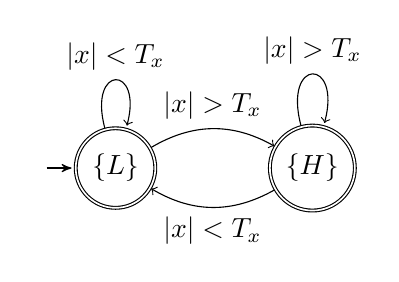
\begin{tikzpicture}[node distance=2.5cm,auto]
    \node (A) [state, accepting, initial] {$\{L\}$};
    \node (B) [state, accepting] [right of=A] {$\{H\}$};
    
    \path[->] (A) edge [loop above] node {$|x| < T_x$} (A);
    \path[->] (A) edge [bend left] node {$|x| > T_x$} (B);
    \path[->] (B) edge [bend left] node {$|x| < T_x$} (A);
    \path[->] (B) edge [loop above] node {$|x| > T_x$} (B);
    %\path[->] (B) edge [bend left] node {$s_{0.7} \wedge est_1$} (A);
    \end{tikzpicture}
}
\def\AutoCompA{
    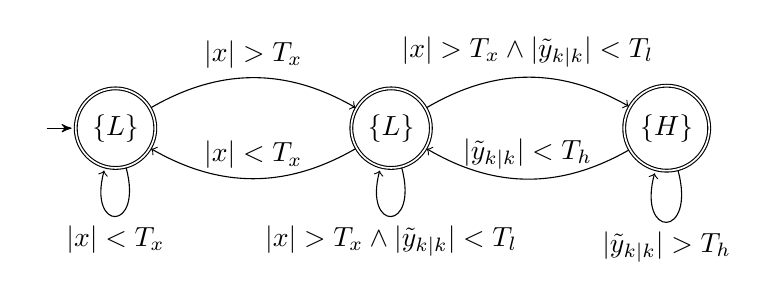
\begin{tikzpicture}[node distance=3.5cm,auto]
    \node (A) [state, accepting, initial] {$\{L\}$};
    \node (B) [state, accepting] [right of=A] {$\{L\}$};
    \node (C) [state, accepting] [right of=B] {$\{H\}$};
    
    \path[->] (A) edge [loop below] node {$|x| < T_x$} (A);
    \path[->] (A) edge [bend left] node {$|x| > T_x$} (B);
    \path[->] (B) edge [bend left, above] node {$|x| < T_x$} (A);
    \path[->] (B) edge [loop below] node {$|x| > T_x \wedge |\tilde{y}_{k|k}| < T_l$} (B);
    
    \path[->] (B) edge [bend left] node {$|x| > T_x \wedge |\tilde{y}_{k|k}| < T_l$} (C);
    \path[->] (C) edge [bend left, above] node {$ |\tilde{y}_{k|k}| < T_h$} (B);
    \path[->] (C) edge [loop below] node {$ |\tilde{y}_{k|k}| > T_h$} (C);
    %\path[->] (B) edge [bend left] node {$s_{0.7} \wedge est_1$} (A);
    \end{tikzpicture}
}
\def\AutoCompB{
    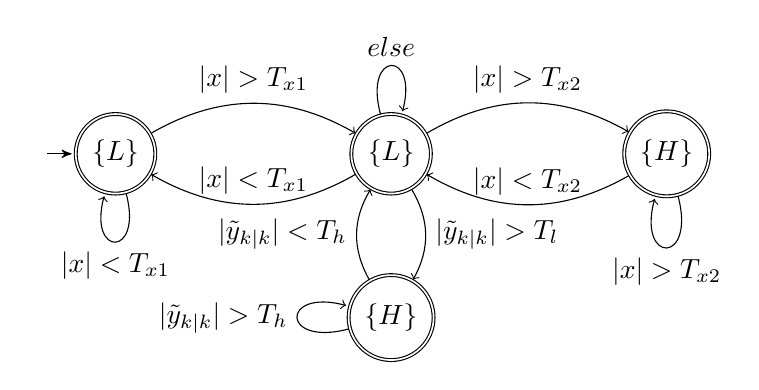
\begin{tikzpicture}[node distance=3.5cm,auto]
    \node (A) [state, accepting, initial] {$\{L\}$};
    \node (B) [state, accepting] [right of=A] {$\{L\}$};
    \node (C) [state, accepting] [right of=B] {$\{H\}$};
    \node (D) [state, accepting] [below=1cm of B] {$\{H\}$};
    
    \path[->] (A) edge [loop below] node {$|x| < T_{x1}$} (A);
    \path[->] (A) edge [bend left] node {$|x| > T_{x1}$} (B);
    \path[->] (B) edge [bend left, above] node {$|x| < T_{x1}$} (A);
    
    \path[->] (B) edge [loop above] node {$else$} (B);
    
    \path[->] (B) edge [bend left] node {$|x| > T_{x2}$} (C);
    \path[->] (C) edge [bend left, above] node {$|x| < T_{x2}$} (B);
    \path[->] (C) edge [loop below] node {$|x| > T_{x2}$} (C);
    
    \path[->] (B) edge [bend left] node {$|\tilde{y}_{k|k}| > T_l$} (D);
    \path[->] (D) edge [bend left] node {$|\tilde{y}_{k|k}| < T_h$} (B);
    \path[->] (D) edge [loop left] node {$|\tilde{y}_{k|k}| > T_h$} (D);
    \end{tikzpicture}
}
\frame{
    \frametitle{Experiment Setup}
    \begin{block}{ }
        \todoil{this slide is needed?}
    \end{block}
}
\frame{
    \frametitle{Vision Mode}
    \begin{center}
        \scalebox{0.6}{
            \tikzGPU
        }
    \end{center}
    \begin{block}{ Image resolution switching }
        \begin{itemize}
            \item Change camera resolution in run time adds large \textbf{delay}
            \item Use \textbf{hardware} (GPU resizer) for fast mode switch 
        \end{itemize}
    \end{block}
}
\frame{
    \frametitle{Constant Vision Mode}
    \begin{block}{ Always low quality mode }
        \begin{itemize}
            \item 240p resolution
            \item mean error of 30cm
            \item 2.1\% CPU usage
        \end{itemize}
    \end{block}
    \begin{block}{ Always high quality mode }
        \begin{itemize}
            \item 960p resolution
            \item mean error of 9.5cm
            \item 30\% CPU usage
        \end{itemize}
    \end{block}
}
\frame{
    \frametitle{Manual Mode flight}
    \begin{center}
        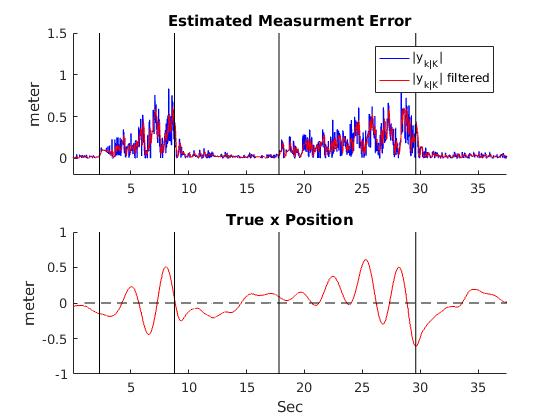
\includegraphics[width=90mm]{errorVsPosition}
    \end{center}
}
\frame{
    \frametitle{Reactive Schedulers}
    \begin{center}
        \begin{columns}
            \hfill
            \begin{column}{5cm}
                \begin{block}{$ A_{err} $ - estimation error based}
                    \scalebox{1}{
                        \AutoErr
                    }
                \end{block}
            \end{column}
            \hfill
            \begin{column}{5cm}
                \begin{block}{$ A_x $ - position based}
                    \scalebox{1}{
                        \AutoX
                    }
                \end{block}
            \end{column}
            \hfill
        \end{columns}
    \end{center}
}
\frame{
    \frametitle{Reactive Schedulers}
    \begin{block}{$$ A_{Comp1} $$}
        \begin{center}
            \scalebox{1}{
                \AutoCompA
            }
        \end{center}
    \end{block}
}
\frame{
    \frametitle{Reactive Schedulers}
    \begin{block}{$$ A_{Comp2} $$}
        \begin{center}
            \scalebox{1}{
                \AutoCompB
            }
        \end{center}
    \end{block}
}
\frame{
    \frametitle{Results}
    \begin{tabular}{m{15em} |  m{4em} | m{5em} }
        \hline
        \textbf{Schedule}& \textbf{\% CPU}  & \textbf{mean($|x|$) (cm)} \\
        \hline
        Only High & 30.9\% & 9.5\\
        \hline
        Only Low & 2.1\% & 30.0\\
        \hline
        $A_{x}$  ($T_x=10$) & \textbf{16.6\%} & \textbf{10.9}\\
        \hline
        $A_{x}$  ($T_x=20$)  & 14.0\% & 14.1  \\
        \hline
        $A_{x}$  ($T_x=30$)  & 8.9\% & 17.4  \\
        \hline
        $A_{err}$ \newline ($T_l=10 , T_h=20$) & 10.3\% & 14.9 \\
        \hline
        $A_{err}$ \newline ($T_l=10 , T_h=15$) & \textbf{11.7\%} & \textbf{11.3} \\
        \hline
        $A_{comp1}$ \newline ($T_x=10$ , $T_l=10$ , $T_h=15$)  &\textbf{ 8.8\%} & \textbf{12.9} \\
        \hline
        $A_{comp2}$ \newline {\footnotesize ($T_{x1}=10$ , $T_{x2}=30$ , $T_l=10$ , $T_h=15$)}   & 10.4\% & 12.7 \\
        \hline
    \end{tabular}
}
\frame{
    \frametitle{Adaptiveness Results}
    \begin{center}
        \AutoErr \\
        $[T_l=10 , T_h=15]$
    \end{center}
    \begin{block}{}
        \begin{tabular}{m{15em} |  m{4em} | m{5em} }
            \hline
            \textbf{conditions}& \textbf{\% CPU}  & \textbf{mean($|x|$) (cm)} \\
            \hline
            Fan off & 11.7\% & 11.3\\
            \hline
            Fan on & 13.2\% & 11.8\\
            \hline
        \end{tabular}
    \end{block}
}
\frame{
    \frametitle{Adaptive Results}
    \begin{center}
        \scalebox{1}{
            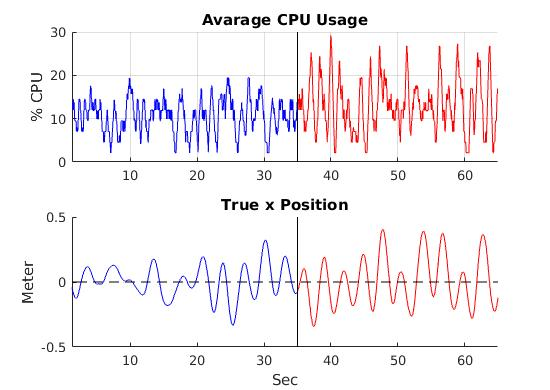
\includegraphics[width=90mm]{windPlot15}
        }
    \end{center}
}



% % % % Conclusion  % % % %
% % % % % % % % % % % % % %
\section{Conclusion}
\subsection{Conclusion}
\frame{
    \todoil{instead of with Related Work}
}
\subsection{Related Work}
\frame{
    \todoil{review of similar papers: A table with few papers}
}

\end{document}
